%Hierarchy is Chapter > Section > Subsection
%http://www.khirevich.com/latex/ - Tips on Writing a Thesis in LaTeX
%This is what to put in the box for bibtex: "/usr/local/texlive/2014/bin/x86_64-darwin/bibtex" %.aux
%Sometimes I might need to run bibtex on its own before doing the full quick build sequence  



\documentclass[a4paper, 11pt, oneside]{report}



%%%% microtype package, for improved typesetting
\usepackage[activate={true,nocompatibility},final,tracking=true,kerning=true,spacing=true,factor=1100,stretch=10,shrink=10]{microtype}
\microtypecontext{spacing=nonfrench}
% activate={true,nocompatibility} - activate protrusion and expansion
% final - enable microtype; use "draft" to disable
% tracking=true, kerning=true, spacing=true - activate these techniques
% factor=1100 - add 10% to the protrusion amount (default is 1000)
% stretch=10, shrink=10 - reduce stretchability/shrinkability (default is 20/20)

%%% other formatting improvement or adjustment packages
\usepackage[margin=1.0in]{geometry} % set the size of all margins in inches
\setlength{\parindent}{0em} % don't indent paragraphs
\setlength{\parskip}{1em} % space between paragraphs

%%% packages that MAY be useful for formatting but are unused unless deemed neccessary
%\usepackage{flushend} % for equalising final page column lengths. messes stuff up sometimes
%\usepackage{setspace}
%\usepackage{pdfpages}
%\hoffset = 9pt
%\voffset = 34pt

%%% font and character packages
\usepackage[T1]{fontenc} % allows for the encoding of unusual or accented characters
\usepackage[bitstream-charter]{mathdesign} % font package similar to the Elsevier font, with included maths style
\usepackage{physics} % provides a family of vector notation

%%% citation packages
\usepackage[nottoc]{tocbibind} % puts the references section into the table of contents
\usepackage{cite} % an alternative to biblatex, it still calls bibtex but unlike bibtex the citation style is defined in the line at the end of the document
\usepackage{url}

%%% packages that provide or position specific elements
\usepackage{datetime} % allows a customised was of writing the date
\usepackage{multirow} % for splitting rows inside tables
\usepackage{float} % for positioning the nomenclature floating tables
\usepackage{subcaption} % allows for captions for sub-figures

%%% packages for handling various graphics files - it seems like three of these may be doing the same thing, and should be consolidated at the end if possible
\usepackage{color} % lets text be different colours
\usepackage{graphics} % for pdf, bitmapped graphics files
\usepackage{epsfig} % for  encapsulated postscript graphics files, a type of vector image
\usepackage{epstopdf} % allows LaTeX to include EPS files by converting each one to a PDF of the same dimensions

%for when David wants a double-spaced version
\linespread{2.5}

%for commenting out sections
\usepackage{comment}



\newdateformat{mydate}{\monthname[\THEMONTH] \THEYEAR}
\title{Sensitivity of\\Nozzle Guide Vane Flow Capacity\\to Geometric Changes}
\author{Tom Franklyn Gammage}
\date{\mydate\today}



\begin{document}



\maketitle

\chapter*{Thanks}

\chapter*{Abstract}

\tableofcontents
\listoffigures
\listoftables

\chapter*{Nomenclature}
\subsection*{Romans}
\subsection*{Greeks}
\subsection*{Acronyms and Abbreviations}
\subsection*{Subscripts}



\chapter{Introduction}
%--Include some derivation of how capacity prediction errors can cause exponentially increasing errors in later stages
%--In the relevant chapter, extend capacity to 2D to show how it becomes more nuanced

%definition is done and good. next steps to add:

%--we know that geometry and pr are the ONLY drivers of Aeff, but we don't know HOW geometry drives changes.

\section{Motivation}

Jet engines are not perfect. Contemporary analysis does not provide a complete understanding of the phenomena by which turbomachinery flows differ from 1-dimensional compressible flow. Contemporary engineering does not provide a realisation of the best performing engine that could be built, but is instead limited by the capabilities of technology. It will be shown that our analytical needs and our performance needs are tied together by our need to predict the engine core mass flow rate as accurately as possible.

The requirement for an accurate core mass flow rate prediction is illustrated by consideration of the Brayton thermodynamic cycle, which is plotted in Figure~\ref{fig:brayton_cycle_plots}.

\begin{figure}[H]
	\centering
	\begin{subfigure}{.45\textwidth}
		\centering
		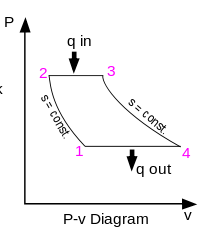
\includegraphics[width=\linewidth]{figs/brayton_cycle_pv_plot.png}
		\caption{p-v plot}
		\label{fig:brayton_cycle_pv_plot}
	\end{subfigure}
	\hspace{0.05\textwidth}
	\begin{subfigure}{.45\textwidth}
		\centering
		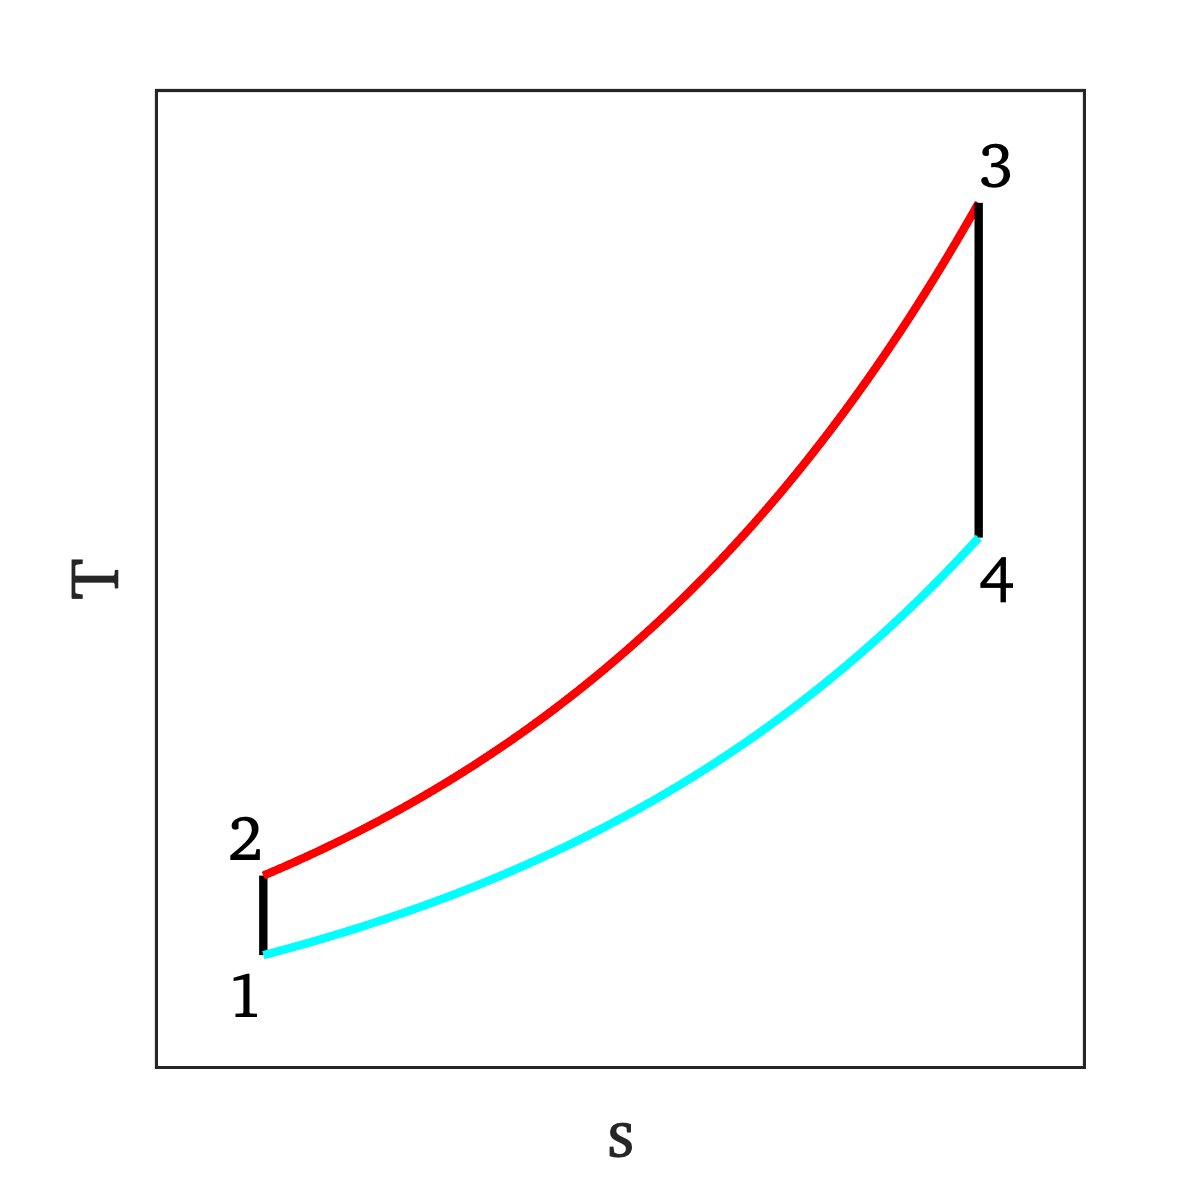
\includegraphics[width=\linewidth]{figs/brayton_cycle_ts_plot.png}
		\caption{T-s plot}
		\label{fig:brayton_cycle_ts_plot}
	\end{subfigure}
	\caption{$p$-$v$ and $T$-$s$ plots of the Brayton thermodynamic cycle}
	\label{fig:brayton_cycle_plots}
\end{figure}

Basic analysis of the Brayton cycle shows that its thermal efficiency is equal to
\begin{equation}
	\eta_{th} = 
	1 - 
	\left(
		\frac{p_{1}}{p_{2}}
	\right)
	^
	\frac{\gamma-1}{\gamma}
\end{equation}
For maximum thermal efficiency, it is thus desirable to maximise the pressure increase produced by the engine's compressor, which is responsible for the process of isentropic compression between stations $1$ and $2$. The compression ratio is limited in practice by the pressure increase that is achievable by contemporary compressors, which must balance the goal with the avoidance of stall, the need for a wide range of operating conditions, and the avoidance of excess complexity from adding additional spools. Cruise-condition compression ratio is thus a design specification which sets the value of $p_2$.

The engine's combustor is responsible for the process of isobaric heat addition between stations $2$ and $3$. The rate of heat addition to the flow is given by
\begin{equation}
	Q_{23} = 
	\dot{m}
	c_p
	\left(
		T_3 - T_2
	\right)
\end{equation}
where $\dot{m}$ is the mass flow rate through the combustor. For the purpose of illustration, the influences of bleed and cooling air mass flow rate are not considered, and $\dot{m}$ is taken to be the mass flow rate through the engine compressor, combustor, nozzle guide vanes, and turbine. $c_p$ is the specific heat of air at constant pressure and $T_2$ is derived from the compressor inlet temperature $T_1$ via isentropic compression as
\begin{equation}
	T_2 = 
	T_1
	\left(
		\frac{p_2}{p_1}
	\right)
	^
	\frac{\gamma-1}{\gamma}
\end{equation}
combining to express the heat added as
\begin{equation}
	Q_{23} = 
	\dot{m}
	c_p
	\left[
		T_3 - 
		T_1
		\left(
			\frac{p_2}{p_1}
		\right)
		^
		\frac{\gamma-1}{\gamma}
	\right]
\end{equation}
For maximum power, it is desirable to maximise the heat added to the flow, which would result in an increase in in $T_3$. A technological limitation is once again presented: the maximum $T_3$ is limited by the avoidance of overheating the post-combustor nozzle guide vanes, for which heat management is of prime concern to the field. $T_3$ is thus a design specification.

Heat addition is well controlled for in contemporary lean-burn engines, where it may be modelled by the relationship
\begin{equation}
	Q_{23} = 
	\eta_h
	H_{LV}
	\dot{m_f}
\end{equation}
where $\dot{m_f}$ is the fuel mass flow rate, $H_{LV}$ is the lower heating value of jet fuel and $\eta_h$ is a constant to account for inefficiencies of heat addition beyond the scope of the present illustration. The above equations combine to show that the required fuel mass flow rate may be modelled by the expression
\begin{equation}
	\frac{\dot{m_f}}{\dot{m}}
	=
	\frac{c_p}{\eta_{h}H_{LV}}
	\left(
		T_3 - 
		T_1
		r_p
		^
		\frac{\gamma-1}{\gamma}
	\right)
\end{equation}
where $r_p$ is the compression ratio, $\frac{p_2}{p_1}$. It is shown that the core mass flow rate, $\dot{m}$, must be accurately predicted if the engine is to be accurately maintained at the optimal operating conditions allowed by its construction. $r_p$ and $T_3$ are known design specifications, $T_1$ is a measurable ambient condition, and all other terms are approximately constant. 

The design of any jet engine depends on the assumption that accurate prediction of $\dot{m}$ is possible. It has been shown that this is directly tied to the performance and operational margins of the upstream engine components. Predictability of $\dot{m}$ also affects the design of every downstream turbine stage. If it differs from its expected value due to a poor prediction, all subsequent turbine stages will be sized for an incorrect mass flow rate. The resulting errors in flow velocity and pressure will compound with each additional stage, leading to increasingly incorrect specification of turbine sizes and turning angles.

Andrea Guiffre' and Matteo Pini~\cite{guiffre_design_guidelines} performed numerical analysis to discuss scaleable guidelines for turbine stage design, validating their model using high-fidelity CFD.  Correct stage matching was found to be highly dependent on matching the \textit{volumetric flow ratio}, defined by the authors as a stage's total-to-static density ratio. To accurately quantify this parameter within the analytical and computational methods discussed in this thesis, mass flow rate would need to be predicted correctly.

A strong understanding of NGV mass flow rate predictability should allow engine-makers to pre-empt geometric changes that happen to NGVs during service, such as erosion and cooling hole blockage. It should also account for geometric uncertainties arising from the manufacturing process. While this study advocates for improved accuracy of capacity predictions, emphasis is placed on how these predictions are limited by the unpredictability of real-world manufacture and service.

Section~\ref{flow_capacity_background_definition_and_derivation} will outline the analysis involved in parameterising and predicting mass flow rate. The section will also present the alternative metric of \textit{flow capacity} as a more useful way of characterising mass flow rate independently of the NGV upstream total pressure and temperature. Defining a purely geometric mass flow rate capacity allows for experimental testing of NGVs without recreating the extreme boundary conditions to which real NGVs are exposed. Setting the correct pressure ratio is sufficent, as the subsequent derivation will show. This expedites the testing of different NGV geometries' effects on mass flow rate.

\section{Flow capacity: background, definition, and derivation}
\label{flow_capacity_background_definition_and_derivation}

The capacity of an internal combustion engine is an intuitive concept. It is simple to derive from the engine's geometry, it has tangible units of volume, and it provides an heuristic for the engine's size, performance, and air mass flow rate. The design of turbomachinery invites an analagous concept to that of IC engine capacity, but a definition is not so obvious. Mass flow rate through an engine's nozzle guide vane is a function of the NGV's geometry and of its boundary conditions. If the mass flow rate can be quantified in a way which mitigates the boundary conditions, then the effects of an NGV's geometry on its mass flow rate may be isolated. A particular NGV will thus have a mass flow rate capacity, just as a particular IC cylinder has a volumetric capacity.

In 1 dimension, an engine nozzle may be modelled as a compressible flow from an upstream reservoir of total pressure $p_0$, accelerating to velocity $v$ and density $\rho$ through a nozzle of cross-sectional area $A$. Mass flow rate through the nozzle is thus
\begin{equation}
\dot{m} = \rho A v
\end{equation}
where density may be expressed as a function of \textit{pressure ratio}, the ratio of the nozzle pressure to the total pressure
\begin{equation}
\rho = \frac{p_0}{R T_0} \left(\frac{p}{p_0}\right)^\frac{1}{\gamma}
\end{equation}
and velocity is given by the compresssible form of Bernouilli's equation as
\begin{equation}\label{compressible_bernouilli}
v =
\sqrt[•]{ 
	2 \left( \frac{\gamma}{\gamma - 1} \right) \left[ \frac{p_0}{\rho_0} - \frac{p}{\rho} \right] 
}
\end{equation}

The above equations combine to express mass flow rate through the nozzle as
\begin{equation}
\dot{m} =
A
\frac{p_0}{R T_0}
\left(\frac{p}{p_0}\right)^\frac{1}{\gamma}
\sqrt[•]{ 
2 \left( \frac{\gamma}{\gamma - 1} \right) 
\left[ \frac{p_0}{ \left( \frac{p_0}{R T_0} \right) } - \frac{p}{ \left( \frac{p_0}{R T_0} \right) \left(\frac{p}{p_0}\right)^\frac{1}{\gamma} } \right] 
}
\end{equation}
which simplifies to
\begin{equation}
\dot{m} =
A
\frac{p_0}{R T_0}
\left(\frac{p}{p_0}\right)^\frac{1}{\gamma}
\sqrt[•]{
	2 \left( 
		\frac{\gamma}{\gamma - 1} 
	\right)
	\left[ 
		R T_0 - R T_0 \left( \frac{p}{p_0} \right)^\frac{\gamma-1}{\gamma} 
	\right]
}
\end{equation}
\begin{equation}\label{mass_flow_rate_formula}
\dot{m} =
\frac{p_0}{\sqrt[•]{T_0}} \>
A \;
\sqrt[]{\frac{\gamma}{R}}
\left(
    \frac{p}{p_0}
\right)^\frac{1}{\gamma}
\sqrt[•]{
	\left(
		\frac{2}{\gamma - 1}  
	\right)
	\left[
		1 - \left( \frac{p}{p_0} \right)^\frac{\gamma-1}{\gamma}
	\right] 
}
\end{equation}

Using $\dot{m}$ from Equation~\ref{mass_flow_rate_formula}, capacity is defined as
\begin{equation}\label{capacity_definition}
\Gamma = \frac{\sqrt[•]{T_0}}{p_0}  \>
\dot{m}
\end{equation}
This provides an expression of mass flow rate independent of upstream total pressure $p_0$ and upstream total temperature $T_0$. The expression is purely a function of throat area $A$ and pressure ratio $\frac{p}{p_0}$:
\begin{equation}
\Gamma =
A \;
\sqrt[]{\frac{\gamma}{R}}
\left(
    \frac{p}{p_0}
\right)^\frac{1}{\gamma}
\sqrt[•]{
	\left(
		\frac{2}{\gamma - 1}  
	\right)
	\left[
		1 - \left( \frac{p}{p_0} \right)^\frac{\gamma-1}{\gamma}
	\right] 
}
\end{equation}

A scale constant $\sigma$ is defined as
\begin{equation}
\sigma = 
\sqrt[]{\frac{2\gamma}{R\left(\gamma-1\right)}} \;
\end{equation}
for a compact expression of capacity as a function of throat area $A$ and pressure ratio $r$:
\begin{equation}
\Gamma \left( A, r \right) = 
\sigma
A \;
\sqrt[]{
	r^\frac{2}{\gamma}
	\left(
		1 - r ^\frac{\gamma-1}{\gamma}
	\right) 
}
\end{equation}
This expression has its maximum value at the critical pressure ratio
\begin{equation}
r_c =
\left(
	\frac{\gamma+1}{2}
\right)
^\frac{\gamma}{1-\gamma}
\end{equation}
At lower ratios, the nozzle is choked and mass flow rate cannot increase further. Choked capacity is given by
\begin{equation}
\Gamma_c \left( A \right) =
\sqrt[]{\frac{2\gamma}{R\left(\gamma-1\right)}}
A \;
\sqrt[]{
	\left(
		\frac{\gamma+1}{2}  
	\right)
	^\frac{2}{1-\gamma}
	\left[
		1 - 
		\left(
			\frac{\gamma+1}{2}
		\right)
		^{-1}
	\right]
}
\end{equation}
which simplifies to
\begin{equation}
\Gamma_c \left( A \right) =
\sqrt[]{\frac{2\gamma}{R\left(\gamma-1\right)}}
A \;
\sqrt[]{
	\left(
		\frac{\gamma+1}{2}  
	\right)
	^\frac{2}{1-\gamma}
	\left[
		\frac{\gamma+1}{\gamma+1}
		-
		\left(
			\frac{2}{\gamma+1}
		\right)
	\right]
}
\end{equation}
\begin{equation}
\Gamma_c \left( A \right) =
A \;
\sqrt[]{
	\frac{2\gamma}{R}
	\left(
		\gamma+1
	\right)
	^\frac{2}{1-\gamma}
	\frac{1}{\gamma+1}
	\left(
		\frac{1}{2}
	\right)
	^\frac{2}{1-\gamma}
}
\end{equation}
\begin{equation}\label{choked_capacity_from_area}
\Gamma_c \left( A \right) =
A \;
\sqrt[]{
	\frac{\gamma}{R}
}
\left(
	\frac{\gamma+1}{2}
\right)
^\frac{1+\gamma}{2\left(1-\gamma\right)}
\end{equation}

It is shown that the capacity of one-dimensional nozzle flow is a function of only the flow's minimum area, provided the flow is choked and the ratio of specific heats is assumed constant. 

Section~\ref{research_structure} will introduce the structure of the following chapters, which are to analyse the capacity of 2-dimensional and 3-dimensional nozzle flows, presenting and discussing analytical techniques for applying the 1D capacity equation to 2D and 3D data. In such cases, capacity will be defined by equation~\ref{capacity_definition}.

\section{Research structure}
\label{research_structure}

The present study seeks to categorise and examine the ways in which nozzle guide vane flow departs from 1-dimensional compressible flow. These departures are numerous and diverse. The study's scope is to include 2 categories of phenomena: difficulties in predicting the mass flow rate through real nozzle guide vanes, and difficulties in quantifying and modelling the loss incurred by various practical solutions to the need for NGV coolant flow.

Although NGV flow capacity is arguably to be maximised in pursuit of greater power, and loss is certainly to be minimised in pursuit of greater efficiency, it is practical to divide efforts according to the areas of NGV engineering where limitations are present. The present study has identified 3 such areas.
\begin{itemize}
	\item NGV casting processes causing variations in overall shape and throat area, limiting the predictability of flow capacity.
	\item Trailing edge machining processes causing variations in trailing edge shape, resulting in complex variations in the flow field near the trailing edge flange, with corresponding variations in flow capacity.
	\item Sensitivity of flow capacity to the addition of extra film cooling holes on the NGV leading edge suction side, including sensitivity to their exact location.
\end{itemize}

NGVs are cast to high precision. Chapter~\ref{chapter_geometric_throat_area} will present the variations that nonetheless exist among sets of vanes that are intended to be identical. These variations are shown to affect the NGVs' geometric throat area. The chapter discusses the challenges inherent in finding a definition of throat area that usefuly predicts the flow capacity of an NGV. The effects of 2-dimensional flow phenomena and geometric variations are presented as confounding factors when considering 2D nozzle flow as opposed to 1D. Further complexity is shown to arise when extending analyses to 3D, where 3D CFD data gathered by Rolls-Royce plc are compared to 2D CFD data from the present study.

Chapter~\ref{chapter_trailing_edge} will discuss the other way in which NGV manufacturing introduces geometric variations that reduce capacity predictability, namely the machining of the trailing edge shape. The machining is designed to optimise the trailing edge's aerodynamics, and not necessarily to minimise variations in its shape. The chapter presents 2D CFD analyses of the effects of variable traling edge flange size on the 2D flow field and resulting flow capacity of the NGV. To address the variability of contemporary trailing edge designs and to examine the possibility of thicker trailing edges in the event of novel manufacturing methods, the chapter presents 2D CFD analyses of a flange-less design. This design's loss performance is analysed, informed by a review of various definitions of loss from the literature, where a lack of concensus on a loss definition is demonstrated.

Chapter~\ref{chapter_leading_edge} will analyse the effects of film coolant injection location on both flow capacity and loss. The chapter discusses the possible requirement for an additional suction-side film cooling hole row to be added to NGVs. Given the variability inherent in the process of drilling film cooling holes, justification is given for a 2D CFD study of the effects of hole location on flow capacity and loss, analagous to the variable trailing edge study of Chapter~\ref{chapter_trailing_edge}. A correlation between hole location and flow capacity is analysed, as is the hole location's effect on loss. The chapter also presents a quasi-3D CFD study to demonstrate that 2D CFD (which amounts to a cooling slot) does not accurately model the discharge and mixing phenomena of a row of circular holes.

Literature review will not be the subject of its own chapter. Literature will be reviewed throughout the thesis whenever relevant to the topic under discussion.

\section{Summary of findings}

\textcolor{red}{Write this after you've got the findings.}

\chapter{Geometric throat area}
\label{chapter_geometric_throat_area}
%this chapter is about the definition of throat area and how to measure it

% NEEDED DATA:
% -T900 smooth vanes, 6x 2D CFD solutions at various pressure ratios
% -Not sure where the 3D data came from, can we check this? ie --GOM scan data

%plan for chapter - answer the following questions:
% 1) what does "throat area" MEAN beyond 1D? Is it the smallest area across the nozzle, or is it a line/surface drawn according to real flow features, most likely the M1 line?
% 1) why does it work quite well in 2D, ie what is mostly NOT changing between the geometries (could almost say what is incidentally being controlled for)?
% 2) what starts changing in 3D to the extent that no linear signal is recognisable in the noise?

%the raw data consists of: 
% -some 2D vanes with different geometries, and a bunch of 3D vanes with different geometries. Range of PRs. For each, there is a "throat area".
%it is thus possible to plot: 
% -changes in throat area versus changes in capacity for the 2D family, for any given PR
% -changes in throat area versus changes in capacity for the 3D family, for any given PR
% -capacity trends for the 2D and 3D vanes
%for each solution, it is possible to define:
% -a "true throat area" based on the M1 line being crossed at oblique angles by every streamline
% -certain geometric parameters describing how its shape is different to the shape of its other family members

%"throat area" just means the smallest line or surface that can be drawn in a nozzle - not sympathetic to anything actually happening in the flow. It only really works in 1D.

A 1-dimensional supersonic nozzle is equivalent to a single streamline of variable cross-sectional area. It is possible to solve for the flow conditions throughout the nozzle, provided area is specified as a function of position along the nozzle. The mass flow rate capacity is a function of only the flow's minimum area, as in equation~\ref{choked_capacity_from_area}.

A 2-dimensional nozzle may be modelled as a group of adjacent streamlines, each of which may have dissimilar area functions. The streamlines' minimum areas may not correspond to a straight line across the narrowest part of the nozzle. 

This is illustrated in Figure~\ref{fig:illustration_of_minimum_area} by supposing the division of a 2-dimensional flow into a finite number of streams of finite width. Each stream has an individual point of minimum width where sonic conditions exist, shown as the transition between subsonic flow in blue and supersonic flow in yellow. These sonic points are distributed on a line distinct from the overall passage line of minimum width. The resulting minimum area line is shown in red along with the geometric minimum area line, to illustrate their disparity.

If this concept is extended to infinitesimal streamlines (and the flow is isentropic) each streamline will experience sonic conditions at its point of minimum area, coalescing to form the 2-dimensional sonic line. The effective throat area of a 2-dimensional nozzle is thus the sum of its streamlines' throat areas. This is distinct from the sonic line length, and may be expressed by the integral
\begin{equation}\label{effective_throat_area_integral}
	A_{eff} = 
	\int_{1}^2 \vu*{v} \vdot \vu*{r} dL
\end{equation}
where $\vu*{v}$ is the unit vector of local flow velocity, $\vu*{r}$ is the unit vector perpendicular to the local sonic line, and the integral is performed on the scalar infinitessimal $dL$ over the length of the sonic line, as illustrated in Figure~\ref{fig:illustration_of_equivalent_throat_area_integral}.
 		
\begin{figure}[H]
	\centering
	\begin{subfigure}{.45\textwidth}
		\centering
		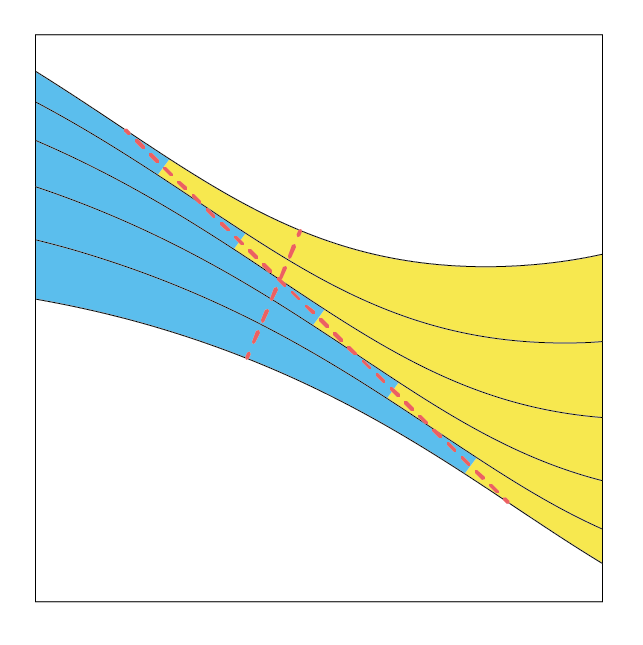
\includegraphics[width=\linewidth]{figs/illustration_of_minimum_area_ver04.png}
		\caption{Different minimum area points of dissimilar streams}
		\label{fig:illustration_of_minimum_area}
	\end{subfigure}
	\hspace{0.05\textwidth}
	\begin{subfigure}{.45\textwidth}
		\centering
		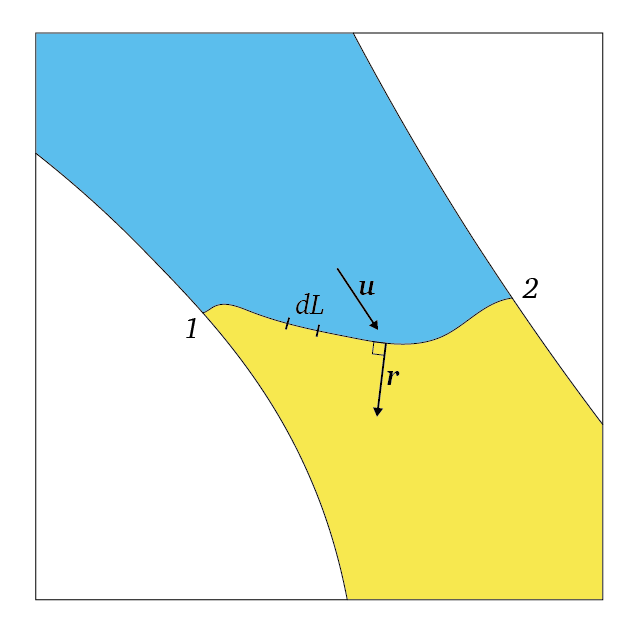
\includegraphics[width=\linewidth]{figs/illustration_of_equivalent_throat_area_integral_ver03.png}
		\caption{Integral for 2D nozzle equivalent throat area}
		\label{fig:illustration_of_equivalent_throat_area_integral}
	\end{subfigure}
	\caption{Considerations for defining minimum area}
\end{figure}

In the case of 1-dimensional nozzle flow, Equation~\ref{effective_throat_area_integral} collapses to the value of the throat area. In the case of 2D flow through an arbitrarily shaped nozzle such as a gas turbine nozzle guide vane, the integral describes the infinitesimal sum of the areas encountered by each streamline at the point of sonic conditions. It is proposed as a physically sensible 2D extension of the 1D concept of throat area, as opposed to placing a ruler across the narrowest point of passage to obtain a geometric throat area. 

The present study will nonetheless discuss the reasons for which geometric throat area remains a useful predictor of NGV flow capacity in many cases, as has been noted in the literature. Deepak Thirumurthy et al~\cite{thirumurthy_throat_area} discussed the challenges and uncertainties associated with the accurate matching of an aeroderivative gas generation turbine. The authors' focus was on various means of predicting capacity to facilitate proper matching. 

The authors noted that ``the throat area of any blade or vane row has a strong influence on the overall capacity of the turbine. The vane or blade throat plane...is defined as the plane formed by the smallest passage area normal to the flow path. The effects are of first order when the throat area is changed for the first stage of the turbine.''


\section{1D vs 2D capacity uncertainty}
\label{section_1d_vs_2d_capacity_uncertainty}
%do I have the T900 family at various PRs, or just at the choking PR? Do I actually need other PRs anyway, given that the throat area stuff looks at the vanes when they are choked?
%I have the case files for just the choked conditions, apparently. But this is ok because I have the gamma curves and plots etc, so I can still enhance the thesis by adding some CFD visualisations at choked conditions, showing the M1 line.
%The point is to see how the different NGVs' capacity varies when plotted against various definitions of throat area. The usefulness of each definition will be discussed.

The immediate challenge in quantifying 2D nozzle flow capacity is that analytical approaches are incomplete. If any nozzle's $A_{eff}$ could be inferred from its geometry, it would be possible to investigate the effects of the geometry on the flow capacity to a high degree of accuracy, but the only way to find $A_{eff}$ is to solve the flow computationally to obtain the $M=1$ line. Once a CFD solution has been obtained, the flow capacity is predicted anyway.

Those concerned with mapping NGV geometry onto flow capacity are thus presented with 2 options: either perform CFD on every conceivable shape of NGV and create a lookup table of arbitrary fidelity, or analyse a relatively small set of CFD solutions to create heuristics about what types of geometric changes cause what types of changes to the shape of the $M=1$ line and local flow vectors.

Rolls-Royce plc have provided the present study with a family of NGV geometries suitable for such an approach, all from the Trent 900 engine. Geometric variation among Trent 900 NGVs has been subject to extensive measurement by Rolls-Royce. In one such set of studies, Terry Hall~\cite{hall_area} and Giulio Zamboni~\cite{zamboni_area} provided geometric definitions of 6 NGVs. These studies considered 2 slightly different production standards within the Trent 900 NGV family, which are referred to by the company as the M-skew standard and the EP1 standard.

Rolls-Royce randomly selected three production NGVs from each standard and measured their surface geometries using the \textit{white light}/\textit{GOM} scanning method. This resulted in the geometric definition files which were provided to the present study by Hall and Zamboni. These files do not include film cooling holes or the trailing edge slot. The trailing edges are smoothly rounded.

%"significant variations" = how many percent - say it here and say it again when talking about 3d area
Significant variations exist among the geometry of the 6 NGVs, even when cooling features are not accounted for. Zamboni described the process for quantifying these variations in 3D, which will be discussed in Section~\ref{2d_vs_3d_capacity_uncertainty}. The present study defined an approach for deriving 2D geometries from the 3D files and quantifying the variations among them.

The 3D NGV surface shape was provided by Rolls-Royce as a set of co-ordinates which define 21 closed loops on the vane surface. Each loop consists of a pair of streamlines which diverge from a stagnation point on the vane's leading edge and converge at the trailing edge. The 11th loop was thus considered to be the closest approximation to a mid-span slice of the NGV.

MATLAB was used to process the 3D curve of the 11th loop, producing a 2D section via the following process. 
\begin{enumerate}
  \item Project the loop's coordinates onto a cylindrical surface whose radius is equal to the NGV annular radius at mid-span.
  \item Periodically repeat the resulting shape in the circumferential direction to create an annulus of 2D vanes wrapped around the cylinder.
  \item Transform the annulus into an infinite 2D linear cascade by taking the circumferential coordinate to be a vertical coordinate.
\end{enumerate}
This process is illustrated in Figure~\ref{fig:2d_geometry_creation}.

\begin{figure}[H]
	\centering
	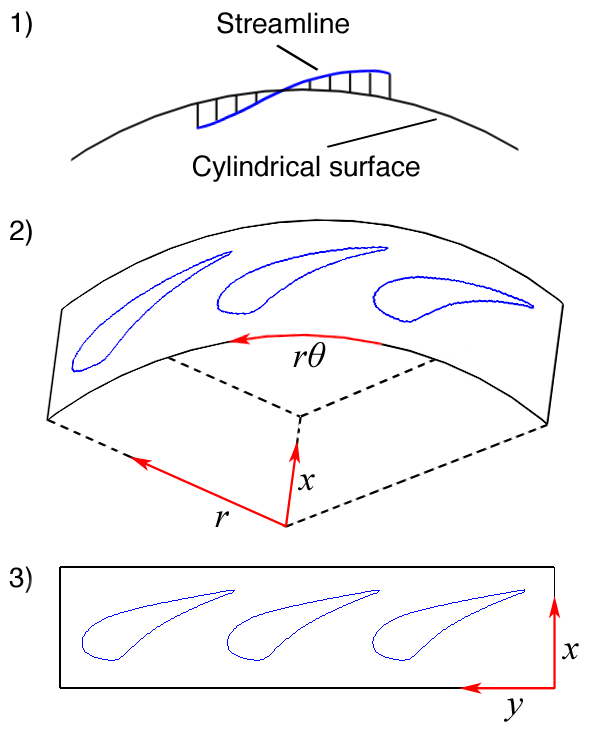
\includegraphics[width=.6\textwidth]{figs/2d_geometry_creation.png}
	\caption{Creation of 2D mid-span approximation of NGV geometry}
	\label{fig:2d_geometry_creation}
\end{figure}

The resulting coordinates were connected to form a closed body. This body was placed in a computational domain consisting of a straight inlet section, a curved turning section, and a straight outlet section inclined at the NGV turning angle. The domain was modelled in Ansys Fluent, where the inlet boundary was specified to have total pressure $p_{01}$ and the outlet was specified to have static pressure $p_2$. The remaining domain boundaries were made periodic with one another to preserve the 2D linear cascade. The NGV surface boundary was specified as a solid wall with a no-slip boundary condition and no heat conduction. The resulting computational domain is illustrated in Figure~\ref{fig:computational_domain_and_boundaries}.

\begin{figure}[H]
	\centering
	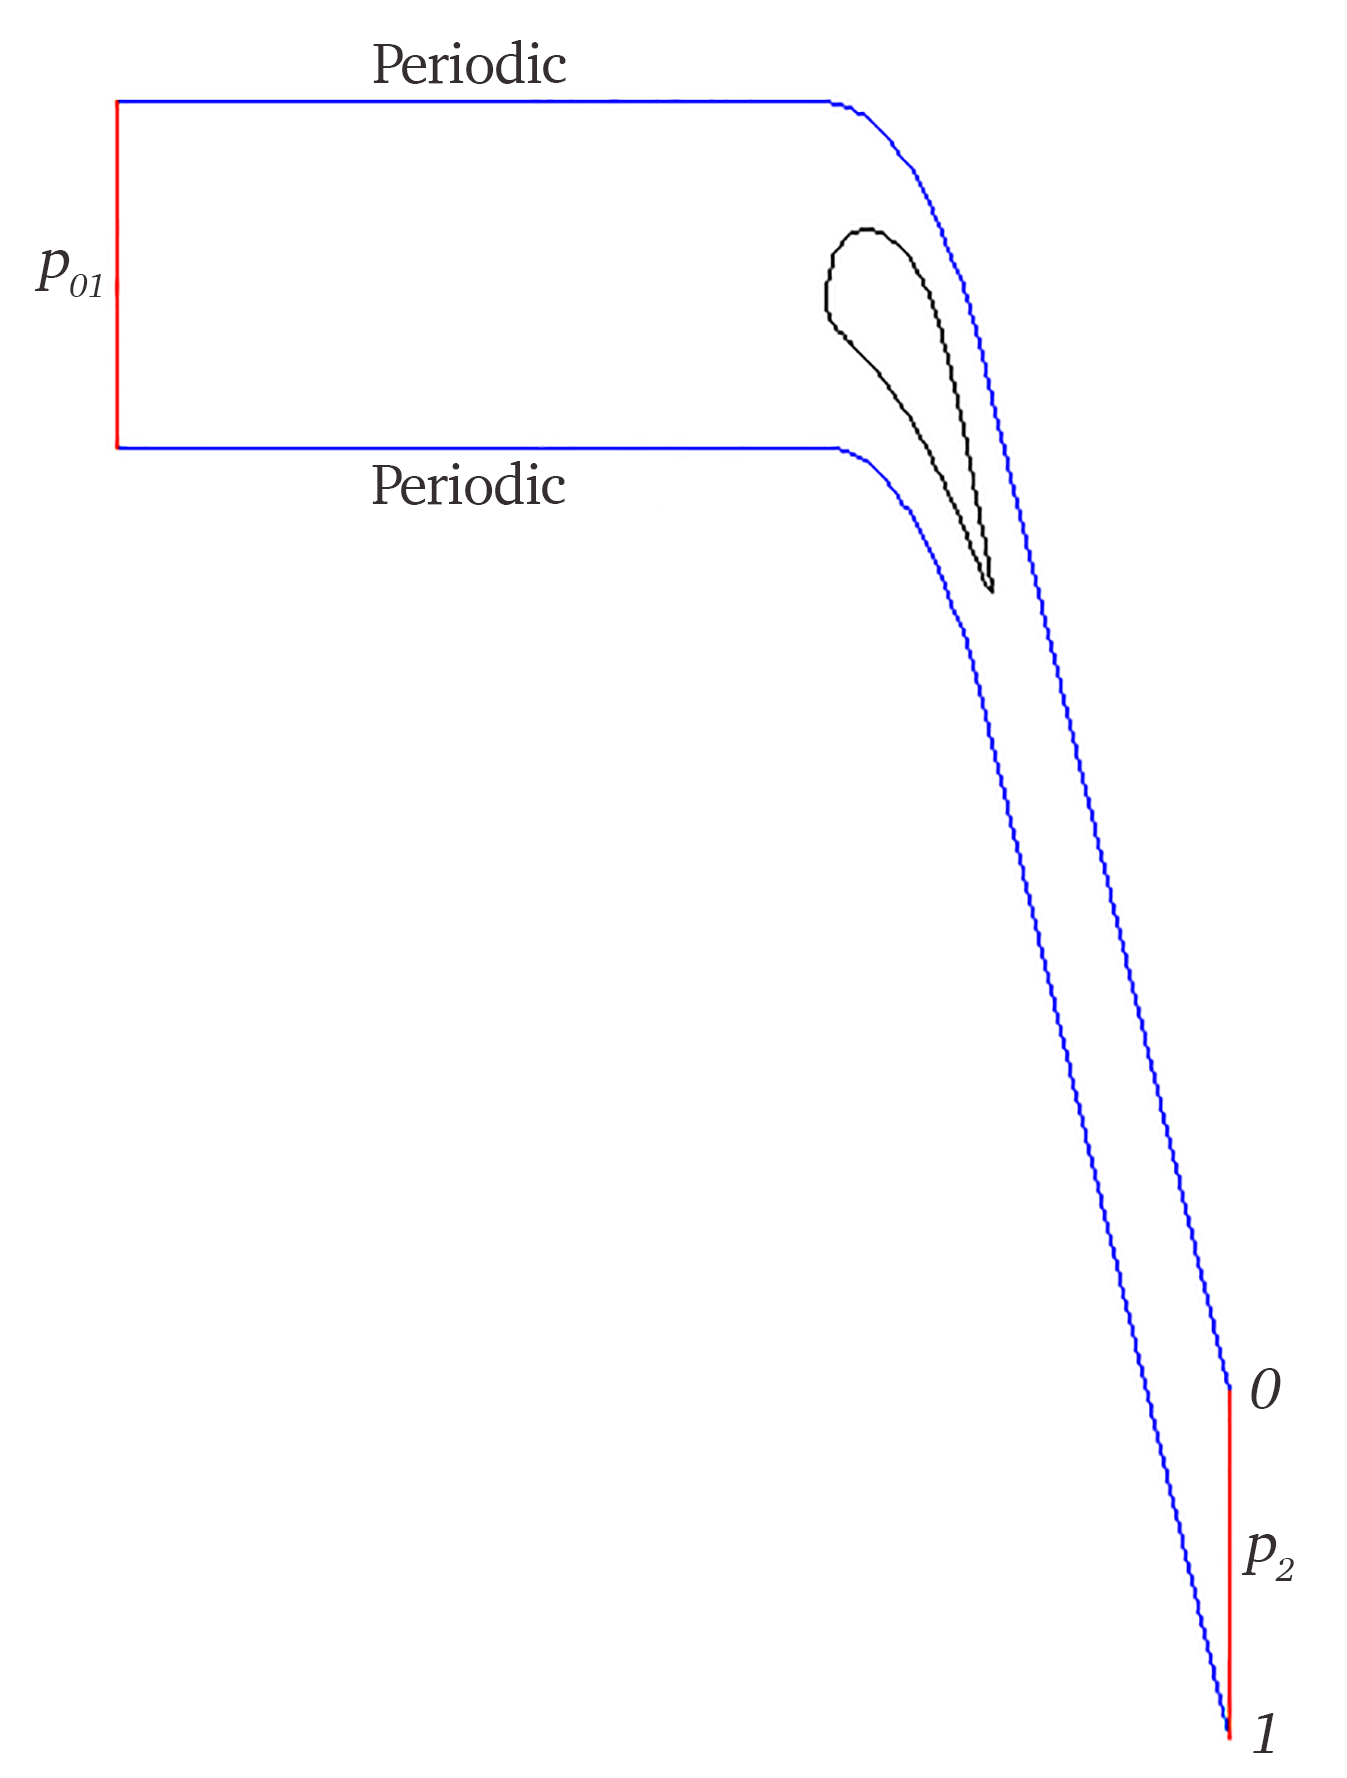
\includegraphics[width=.6\textwidth]{figs/domain_boundary_conditions.png}
	\caption{Computational domain and boundaries}
	\label{fig:computational_domain_and_boundaries}
\end{figure}

This configuration has been the basis for all other 2D CFD analyses in the present study, where additional boundaries are added to account for cooling features as required. Values for the simulation were set according to Table~\ref{T900_parameters}.

% this table's PR checks out. The crazy high pressure ratio on Fluent is just where it finished after going through all the ratios.
\begin{table}[H]
\caption{Boundary conditions at design pressure ratio for multi-vane capacity study}
\label{T900_parameters}
\begin{center}
\begin{tabular}{|c|c|}
\hline
Parameter & Value\\
\hline
NGV series & Rolls-Royce Trent 900\\
NGV turning (degrees) & 76.89\\
Design pressure ratio & 1.79\\
Inlet total pressure (Pa) & $4.33 \times 10^6$\\
Inlet total temperature (K) & 300\\
Outlet static pressure (design) (Pa) & $2.42 \times 10^6$\\
Outlet static temperature (Pa) & 300\\
Solver type & Density-based\\
Cell count & 35,000\\
\hline
\end{tabular}
\end{center}
\end{table}

Matlab was used to calulate the minimum throat width of each 2D NGV. The resulting values are given in Table~\ref{T900_throat_widths}.

\begin{table}[H]
\caption{Throat widths of 6 Trent 900 NGVs}
\label{T900_throat_widths}
\begin{center}
\begin{tabular}{|c|c|c|}
\hline
Production standard & Serial number & Throat width (mm)\\
\hline
\multirow{3}{*}{M-skewed} & KSZ03 & 12.4\\
 & KTA01 & 12.5\\
 & KVD04 & 12.2\\
 \hline
 \multirow{3}{*}{M EP1} & PNN06 & 12.7\\
 & PNS03 & 12.7\\
 & PNS04 & 12.7\\
\hline
\end{tabular}
\end{center}
\end{table}

For turbomachinery flows of this type, the boundary layer thickness will be shown to be large enough to significantly affect the NGV throat area. The mesh must resolve the whole boundary layer within a region of high resolution which is sufficiently large to cover the maximum boundary layer thickness. The maximum thickness of a turbulent boundary layer is approximated by the formula
\begin{equation}\label{boundary_layer_thickness}
\delta \approx
0.37
\frac{L}{Re^\frac{1}{5}}
\end{equation}
where $L$ is the characteristic length in the direction of the flow (the approximate NGV chord length) and $Re$ is the Reynolds number. The Reynolds number is defined as
\begin{equation}
Re = 
\frac{uL\rho}{\mu}
\end{equation}
where $u$ is a representative value for flow velocity and $\mu$ is the dynamic viscosity of the fluid within the temperature range of the flow. For compressible flow, the velocity and denisity are substituted to give
\begin{equation}
Re = 
\frac{
	M\sqrt{\gamma RT}L\frac{p}{RT}
}{
	\mu
}
\end{equation}
which simplifies to
\begin{equation}
Re =
\frac{L}{\mu}
\sqrt{\frac{\gamma}{R}}
\frac{p}{\sqrt{T}}
M
\end{equation}
\begin{equation}
Re =
\frac{L}{\mu}
\sqrt{\frac{\gamma}{R}}
\frac{p_0}{\sqrt{T_0}}
M
\frac{
	\left(
		1 + \frac{\gamma-1}{2}
		M^2
	\right)
	^{-\frac{\gamma}{\gamma-1}}
}{
	\sqrt{
		\left(
			1 + \frac{\gamma-1}{2}
			M^2
		\right)
		^{-1}
	}
}
\end{equation}
\begin{equation}\label{reynolds_number_compressible}
Re = 
\frac{L}{\mu}
\sqrt{\frac{\gamma}{R}}
\frac{p_0}{\sqrt{T_0}}
M
\left(
	1 +
	\frac{\gamma-1}{2}
	M^2
\right)
^{\frac{\gamma+1}{2(1-\gamma)}}
\end{equation}

Equation~\ref{reynolds_number_compressible} was used to compute a Reynolds number for the case of choked or near-choked NGV flow with the following values, based on the values specified in Table~\ref{T900_parameters}.
\begin{table}[H]
\caption{Values for calculating NGV Reynolds number}
\label{reynolds_number_parameters}
\begin{center}
\begin{tabular}{|c|c|}
\hline
Parameter & Value\\
\hline
$L$ & 0.08 m\\
$\mu$ & $19 \times 10^{-6}$ Pas\\
$p_0$ & $4.33 \times 10^6$ Pa\\
$T_0$ & 300 K\\
$\gamma$ & 1.4\\
$R$ & 287 Jkg$^{-1}$K$^{-1}$\\
$M$ & 1\\
\hline
\end{tabular}
\end{center}
\end{table}
This resulted in a value of $Re = 4.2 \times 10^7$. Maximum boundary layer thickness was thus estimated using equation~\ref{boundary_layer_thickness} to be 1 mm. This is of the order of 10\% of the NGV throat width, so full resolution of the boundary layer is required for any CFD study of the effects of NGV geometric changes.

The NGV surface was enclosed in a structured quadrilateral mesh which extended out by 2 mm. Compared to the estimated maximum boundary layer thickness, the factor of 2 ensured that the whole boundary layer was captured, reduced the gradient of cell size change within the boundary layer mesh, and provided additional resolution within the base region downstream of the trailing edge, where boundary layer separation and entropy generation occur amid high surface curvature.

Full resolution of the boundary layer required placement of mesh elements within the laminar sub-layer. Regions within the boundary layer were assumed to be divided according to the \textit{universal law of the wall}. This boundary layer model is derived from experimental measurements and dimensional analysis performed by Johann Nikuradse~\cite{nikuradse_boundary_layers}. The author's motivation was the need to predict the velocity profile and thickness of turbulent boundary layers, given the free-stream conditions. The work is of renewed importance in the context of contemporary CFD such as the present study, where knowledge of appropriate boundary layer mesh resolution is mandatory. 

Nikuradse showed that turbulent boundary layers in general exhibit a high degree of dimensional similarity if distance from the wall $y$ is appropriately non-dimensionalised. The assumption was that qualitatively distinct regions of the boundary layer may be characterised by a dimensionless number that takes the place of $y$. Regions closer to the wall are expected to be dominated by viscous forces, and regions closer to the free-stream are expected to be dominated by inertial forces. The dimensionless wall distance parameter is thus expected to take similar form to the Reynolds number. It is defined as
\begin{equation}\label{y_plus}
y_+ =
\frac{u_f y \rho}{\mu} 
\end{equation}
where $u_f$ is the friction velocity, defined as
\begin{equation}\label{friction_velocity}
u_f = 
\sqrt{
	\frac{\tau_w}{\rho}
}
\end{equation}
where $\tau_w$ is the shear stress at the wall boundary. Equation~\ref{friction_velocity} thus characterises the wall shear stress as a velocity which is used in the Reynolds-type formulation of Equation~\ref{y_plus}. $\tau_w$ is defined as
\begin{equation}\label{wall_shear_stress_definition}
\tau_w =
\frac{1}{2}
C_f
\rho
u^2
\end{equation}
where $C_f$ is a coefficient of skin friction and $u$ is the free-stream velocity. $C_f$ may be computed from the free-stream Reynolds number according to the correlation proposed by Hermann Schlichting~\cite{schlichting_boundary_layer_theory}
\begin{equation}
C_f =
\left(
	2
	\log_{10}
	Re
	-
	0.65
\right)^{-2.3}
\end{equation}

For compressible flows, equation~\ref{wall_shear_stress_definition} may be expressed as
\begin{equation}
\tau_w =
\frac{1}{2}
C_f
\frac{p}{RT}
M^2
\gamma
RT
\end{equation}
\begin{equation}
\tau_w =
\frac{1}{2}
C_f
\gamma
p_0
M^2
\left(
	1 +
	\frac{\gamma-1}{2}
	M^2
\right)
^{-\frac{\gamma}{\gamma-1}}
\end{equation}
allowing a compressible expression of $u_f$ as
\begin{equation}
u_f = 
\sqrt{
	\frac{
		\frac{1}{2}
		C_f
		\gamma
		p_0
		M^2
		\left(
			1 +
			\frac{\gamma-1}{2}
			M^2
		\right)
		^{-\frac{\gamma}{\gamma-1}}
	}{
		\rho_0
		\left(
			1 +
			\frac{\gamma-1}{2}
			M^2
		\right)
		^{-\frac{1}{\gamma-1}}
	}
}
\end{equation}
\begin{equation}
u_f = 
\sqrt{
	\frac{
		C_f
		\gamma
		R
		T_0
		M^2
	}{
		2 +
		\left(\gamma-1\right)
		M^2
	}
}
\end{equation}
and allowing a compressible expression of $y_+$ as
\begin{equation}
y_+ = 
\sqrt{
	\frac{
		C_f
		\gamma
		R
		T_0
		M^2
	}{
		2 +
		\left(\gamma-1\right)
		M^2
	}
}
\frac{y}{\mu}
\frac{p_0}{R T_0}
\left(
	1 +
	\frac{\gamma-1}{2}
	M^2
\right)
^{-\frac{\gamma}{\gamma-1}}
\end{equation}
\begin{equation}\label{y_plus_compressible}
y_+ =
\frac{y}{\mu}
\sqrt{\frac{\gamma}{R}}
\frac{p_0}{\sqrt{T_0}}
\sqrt{\frac{C_f}{2}}
M
\left(
	1 +
	\frac{\gamma-1}{2}
	M^2
\right)
^{\frac{\gamma+1}{2(1-\gamma)}}
\end{equation}
This expression is of similar form to the expression for Reynolds number in equation~\ref{reynolds_number_compressible}. Both are shown to be a function of Mach number and of the upstream conditions $\frac{p_0}{\sqrt{T_0}}$. If these expressions are normalised against the upstream conditions in a similar way to flow capacity, it is shown that both the dimensionless speed $Re$ and the dimensionless boundary layer thickness $y_+$ are purely functions of Mach number and of a geometric parameter -- $L$ and $y$ respectively. This is subject to the assumptions that $\mu$ is approximately constant within the range of temperatures and $\sqrt{\frac{C_f}{2}}$ is approximately constant for sufficiently high Reynolds numbers.

Equation~\ref{y_plus_compressible} may be rearranged to compute a real distance $y$ from the wall given a value of $y_+$. In the general case of turbulent boundary layers, the laminar sublayer occupies the region of $y_+ < 5$. The present study placed the first layer of mesh nodes at a wall distance of 0.3 $\mu$m corresponding to a $y_+$ value of $5$. This is in accordance with a study of laminar sublayer resolution by Salim M. Salim and Siew-Cheong Cheah~\cite{salim_y_plus}.

Within the structured boundary mesh, element size was grown so that the outermost elements had an aspect ratio of approximately $\frac{1}{2}$. Beyond this, the domain was populated with an unstructured quadrilateral-dominant mesh. Node distributions along the two periodic boundaries were made identical, and nodes adjacent to the structured boundary layer mesh were made to match its outermost node distributions. Within the general domain, unstructured mesh generation was automated using Ansys Fluent's built-in meshing feature. The resulting mesh formed the basis for all other 2-dimensional NGV meshes in the study. The mesh and periodic pattern are depicted in Figure~\ref{fig:t900_mesh_whole} and details of the mesh, showing the structured boundary layer treatment, are depicted in Figure~\ref{fig:t900_mesh_details}.

\begin{figure}[H]
      \centering
      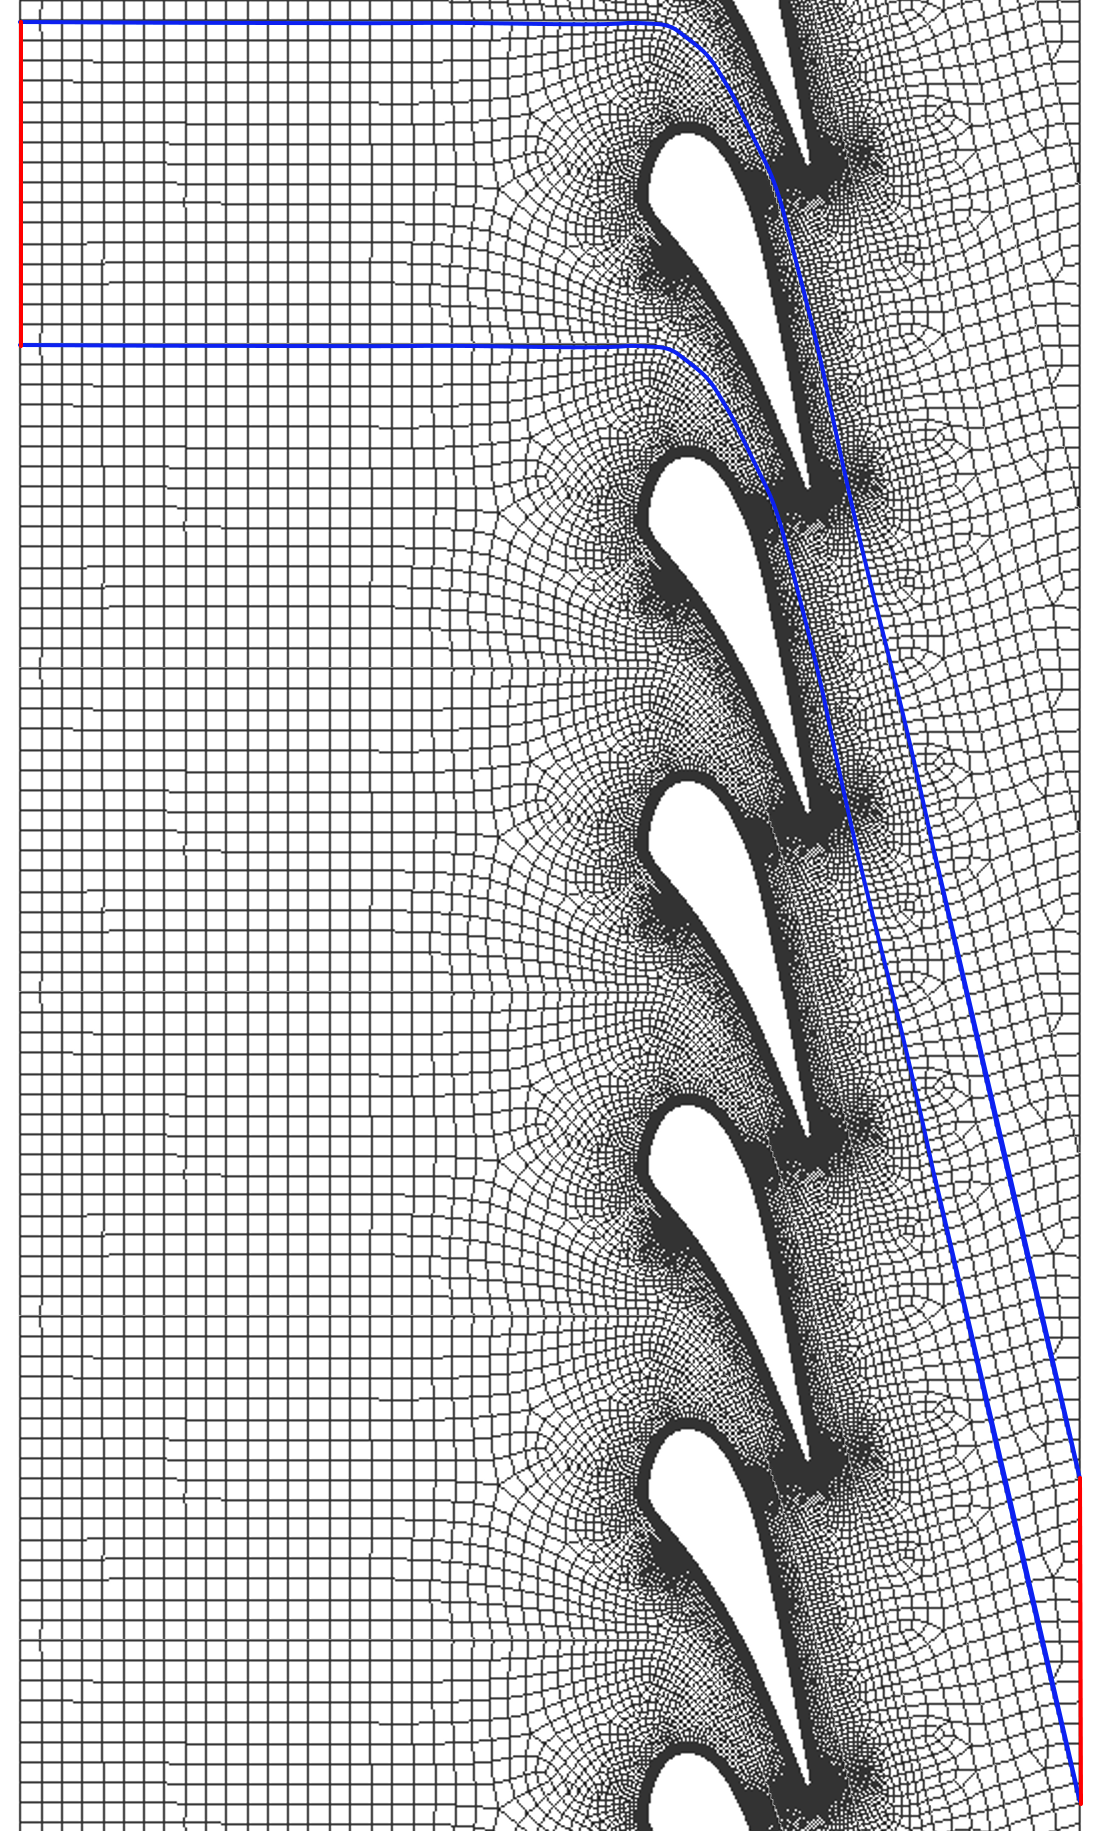
\includegraphics[width=.90\textwidth]{figs/t900_mesh_whole.png}
      \caption{Mesh for T900 throat width variation study}
      \label{fig:t900_mesh_whole}
\end{figure}

\begin{figure}[H]
	\centering
	\begin{subfigure}{.45\textwidth}
		\centering
		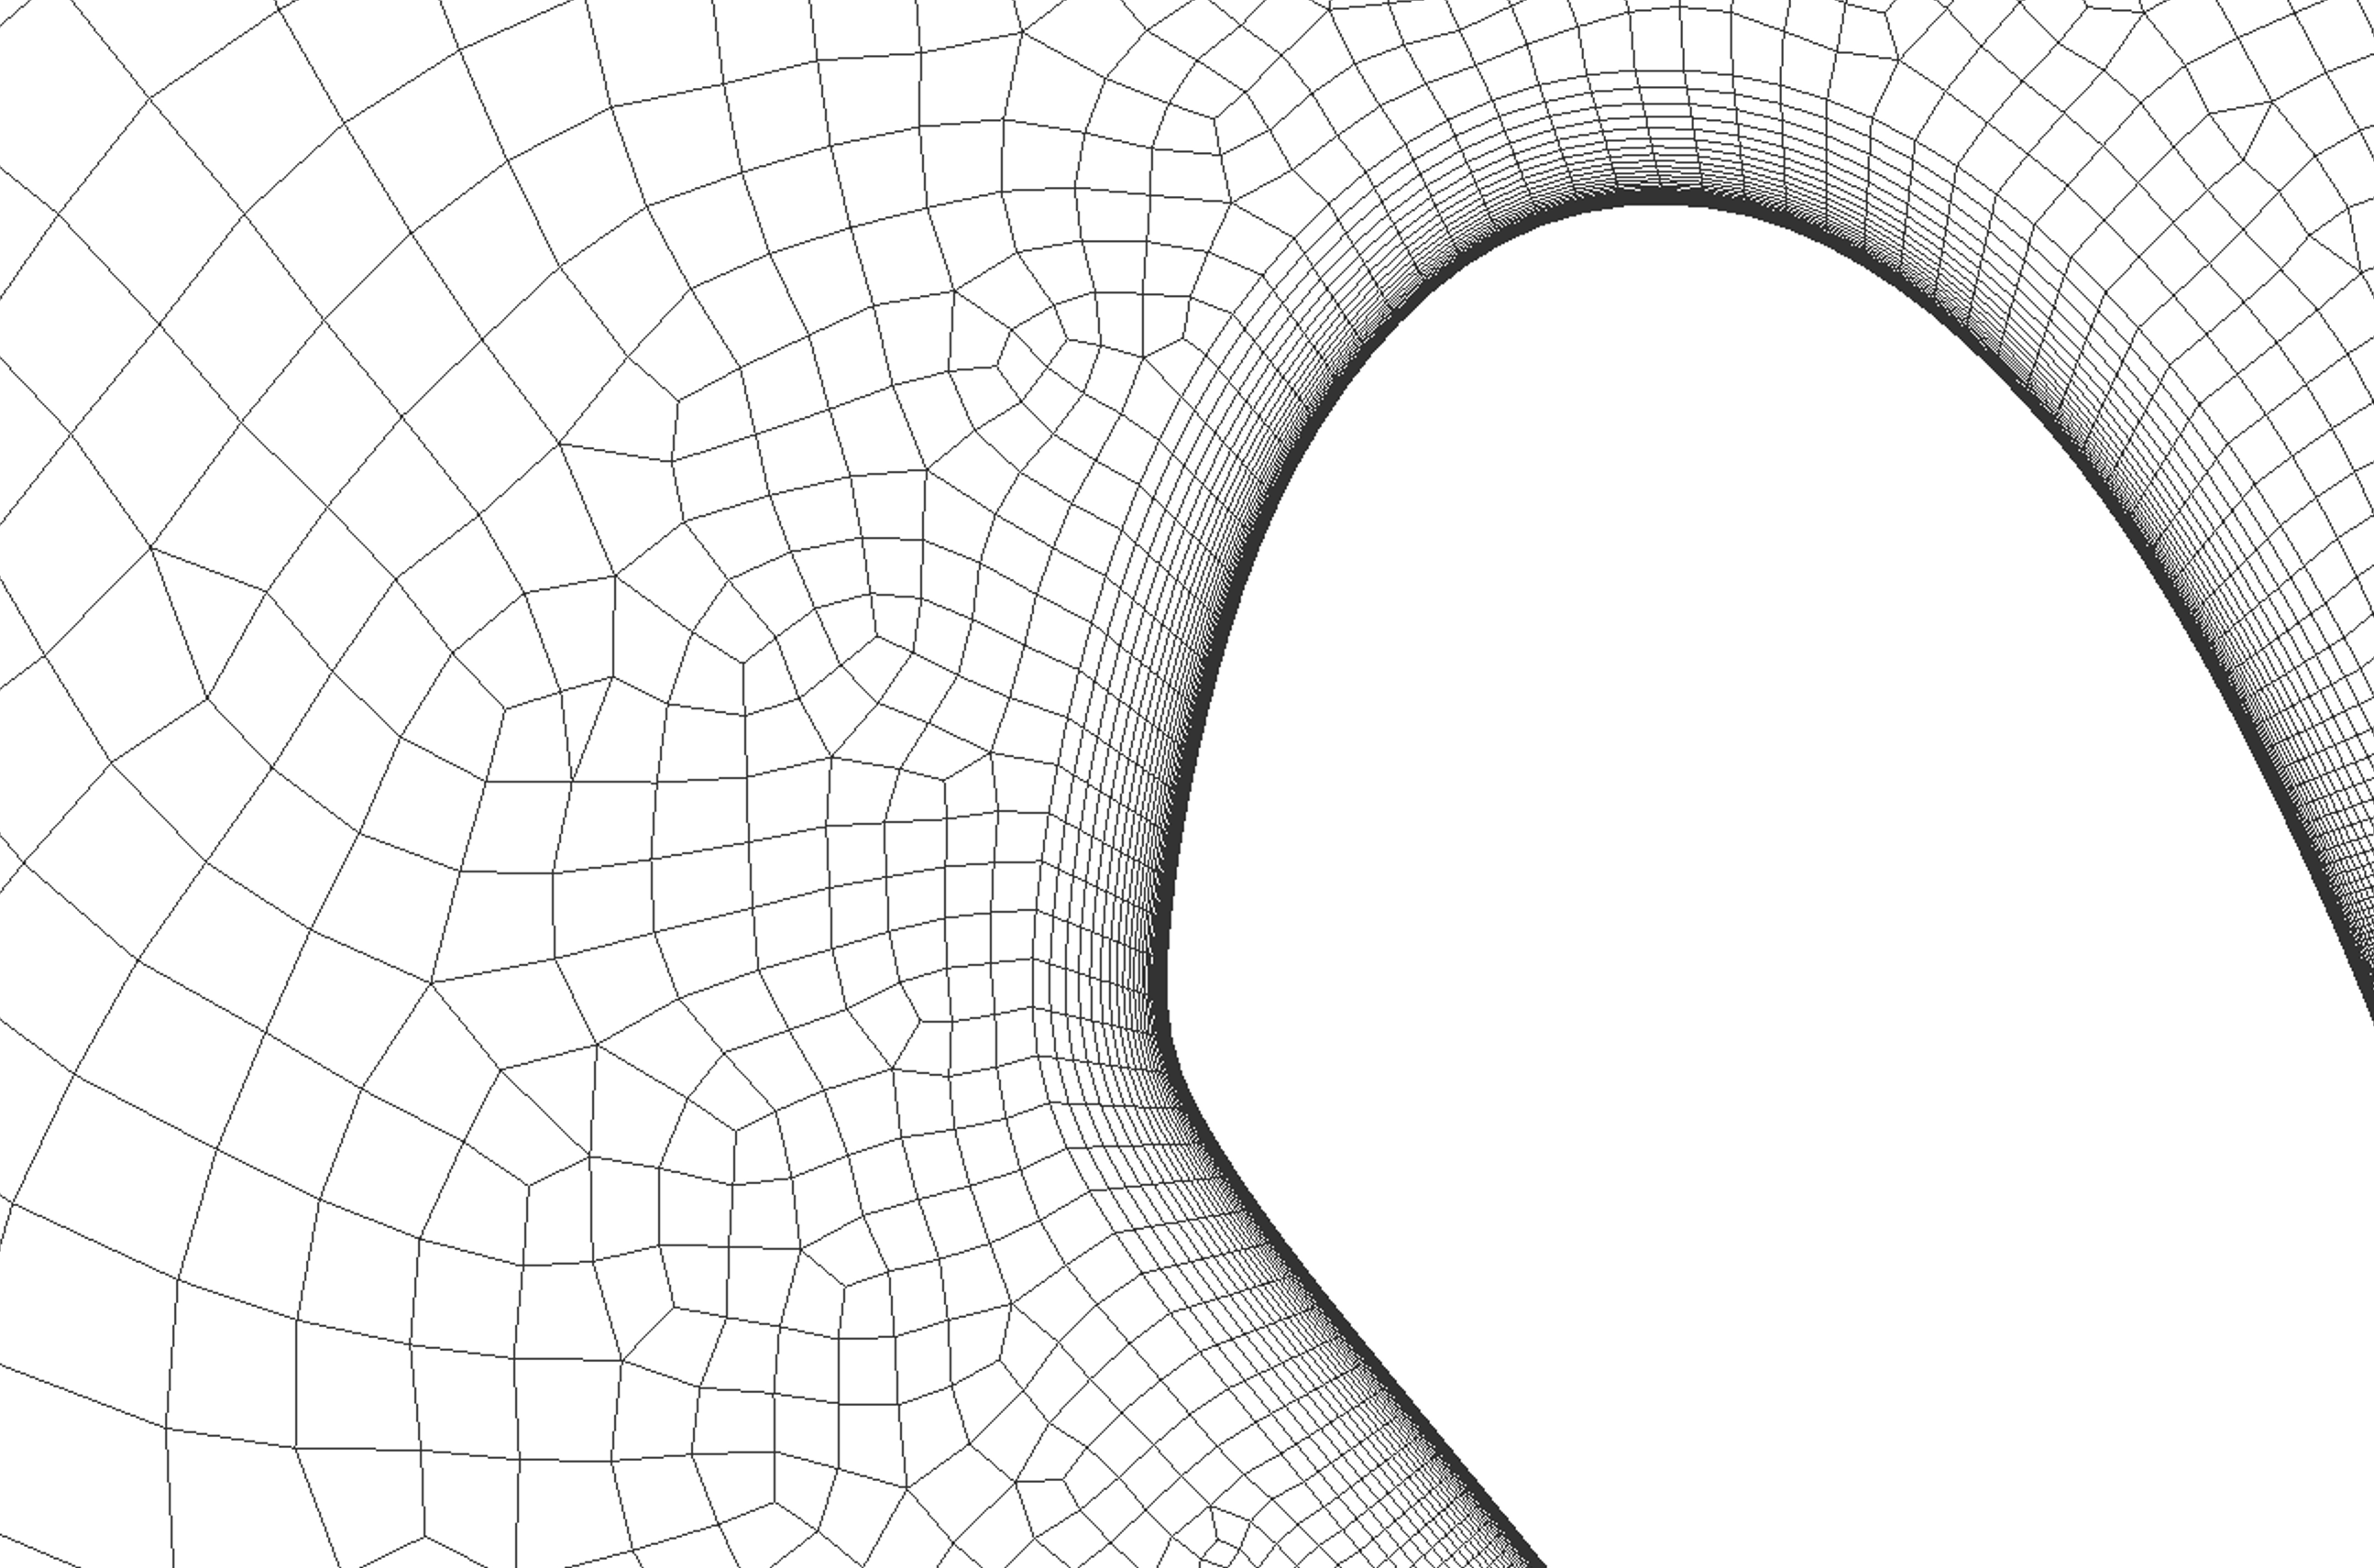
\includegraphics[width=\linewidth]{figs/t900_mesh_leading_edge.png}
		\caption{Leading edge}
		\label{fig:t900_mesh_leading_edge}
	\end{subfigure}
	\hspace{0.05\textwidth}
	\begin{subfigure}{.45\textwidth}
		\centering
		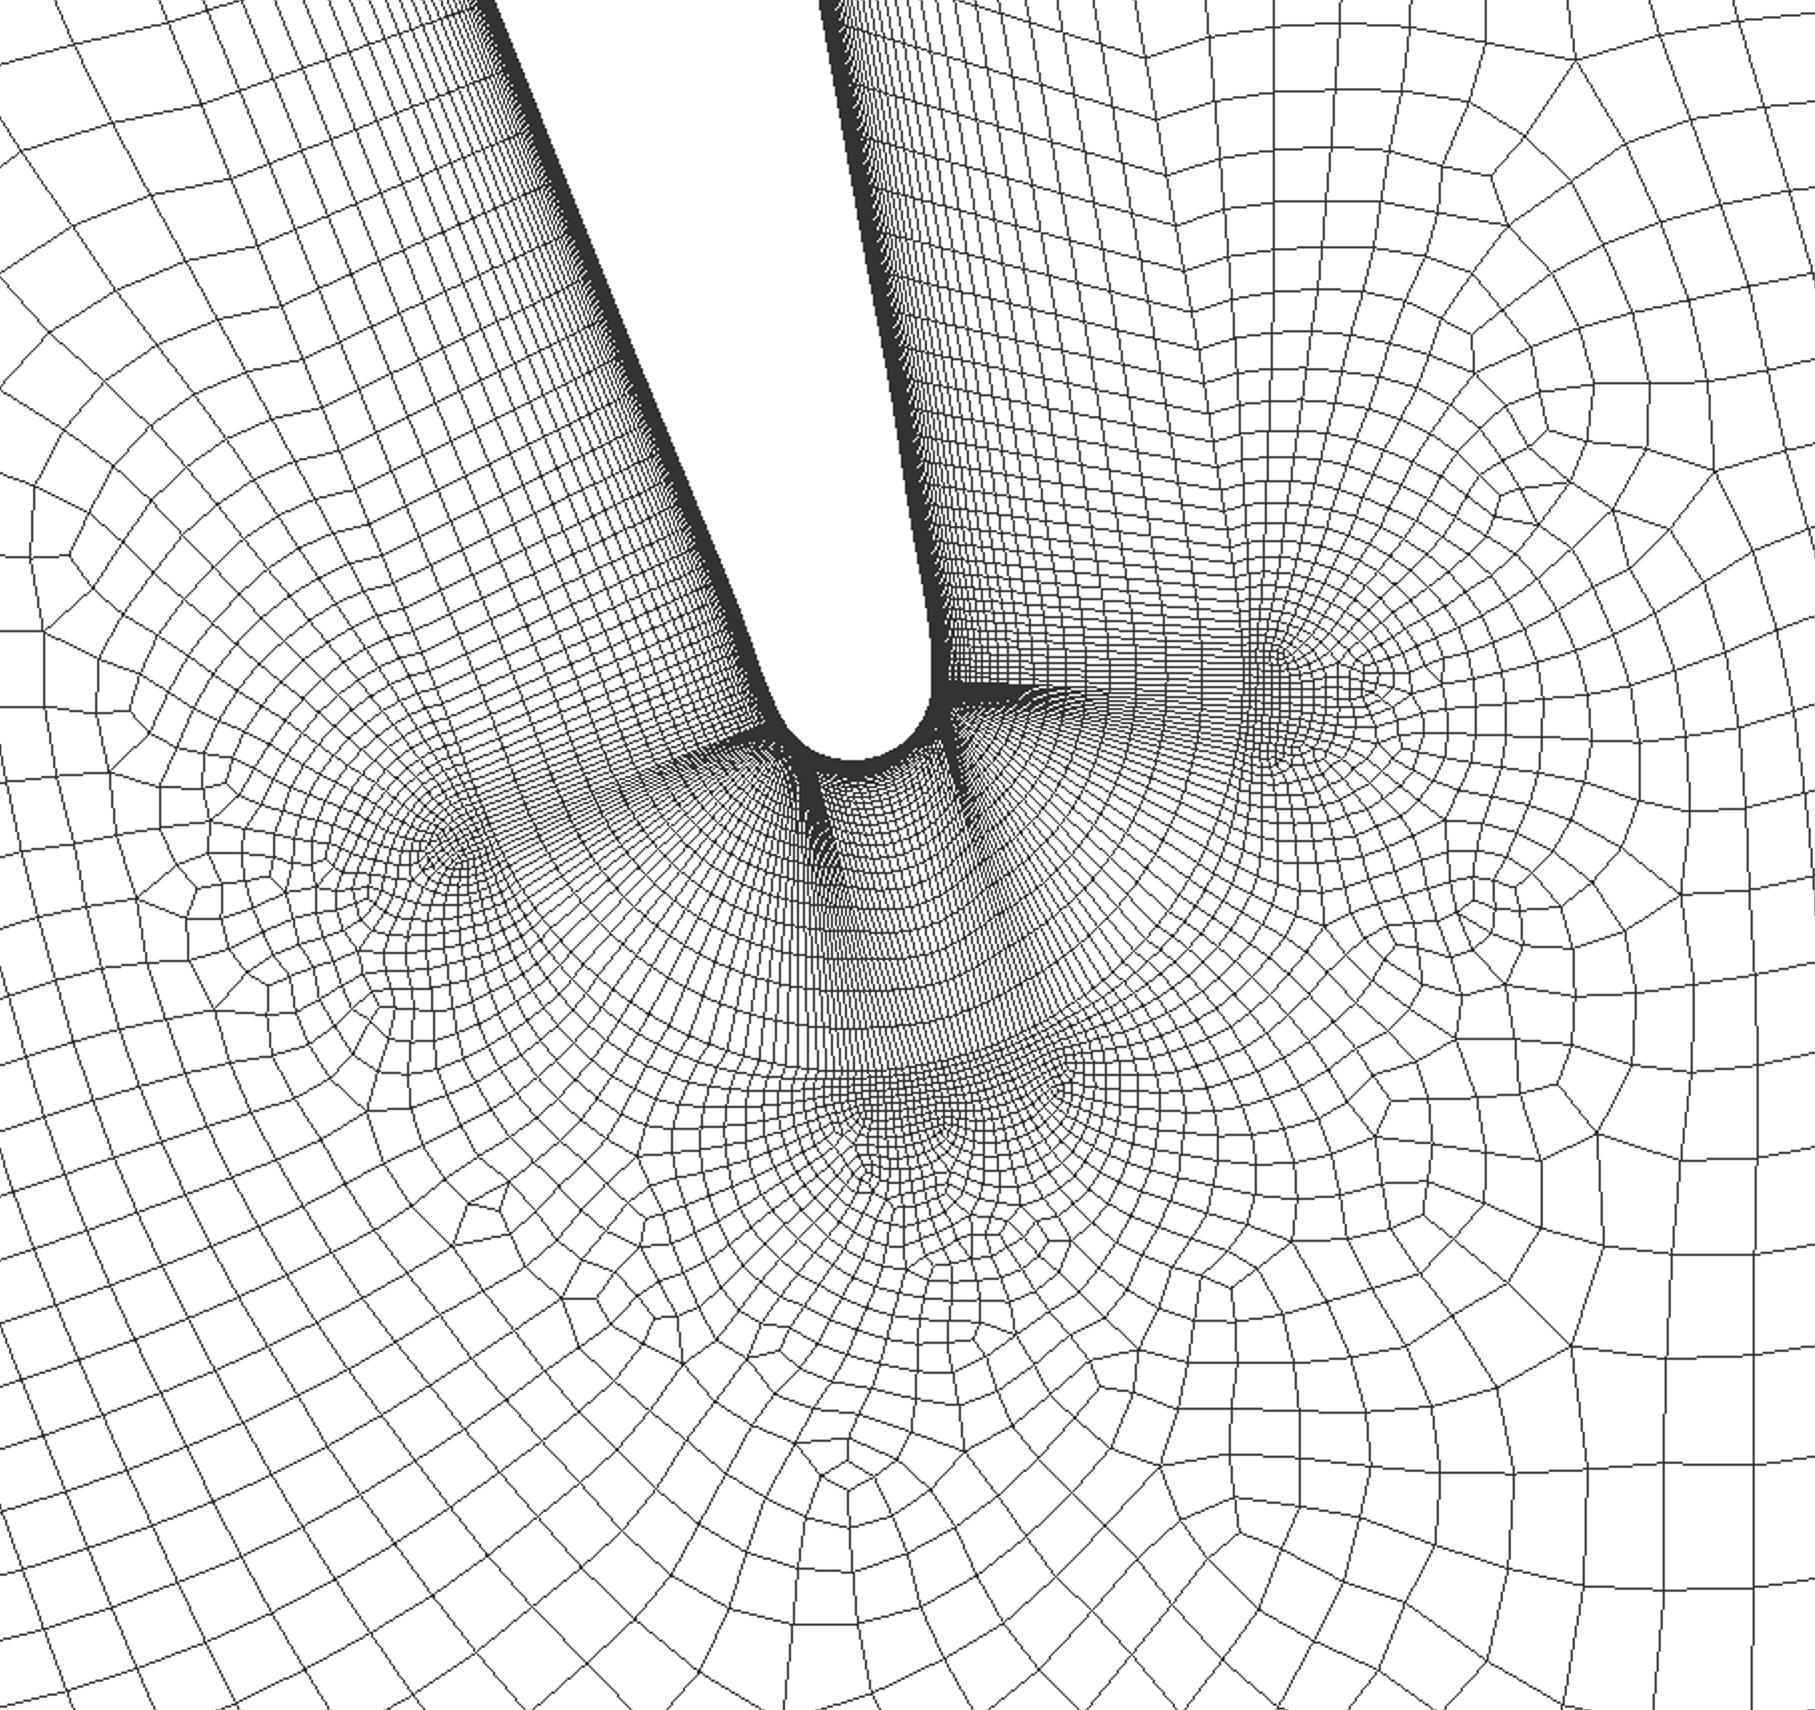
\includegraphics[width=\linewidth]{figs/t900_mesh_trailing_edge.png}
		\caption{Trailing edge}
		\label{fig:t900_mesh_trailing_edge}
	\end{subfigure}
	\caption{Details of mesh for T900 throat width variation study}
	\label{fig:t900_mesh_details}
\end{figure}

The described mesh and boundary condition specifications were used to perform a series of CFD simulations of each of the 6 2D NGVs in Ansys Fluent. Solutions were initialised using the solver's built-in FMG initialisation. This procedure automatically constructs a coarser version of the supplied mesh, on which an initial solution is converged before refinement to the final resolution. More detailed expanation of the scheme is provided by Ansys~\cite{ansys_fmg_initialisation}. A script in the Fluent Journal language was used to produce solutions at incrementally decreasing pressure ratios of between 0.99 and a fully choked pressure ratio of 0.3. NGV mass flow rate was saved at each pressure ratio. Full solution data were saved for the final fully choked pressure ratio to enable analysis of the shocks, expansions and $M=1$ line at choked conditions. There were 32 increments and typical overall solution times were approximately 10 hours. The SST-k$\omega$ turbulence model was used. 

Figure~\ref{fig:t900_mach_whole} shows contours of Mach number for one of the 6 solutions at a fully choked pressure ratio. Figure~\ref{fig:t900_mach_throat} shown contours of Mach number for the same solution in the throat region.

\begin{figure}[H]
      \centering
      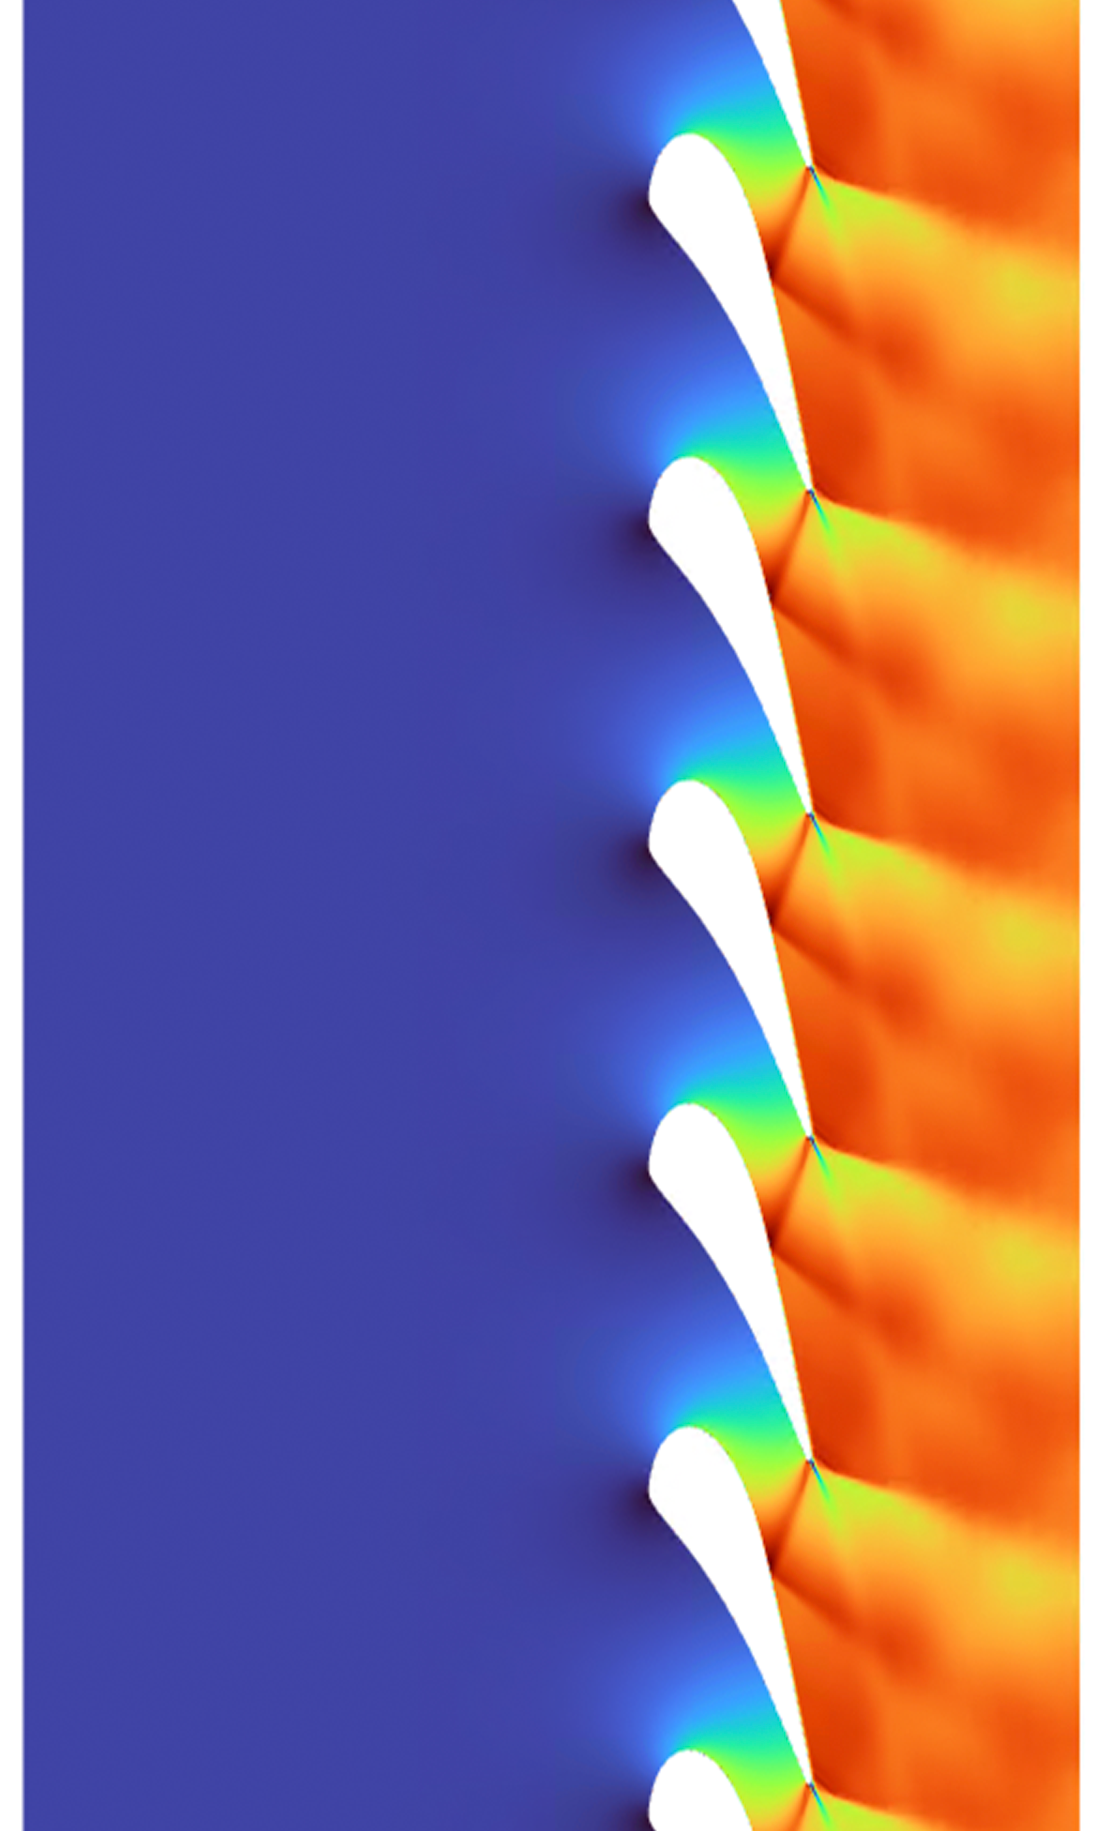
\includegraphics[width=.90\textwidth]{figs/t900_mach_whole.png}
      \caption{Contours of Mach number for  whole solution on vane KSZ03, $\frac{p_{01}}{p_2} = 3.33$}
      \label{fig:t900_mach_whole}
\end{figure}

\begin{figure}[H]
      \centering
      
\includegraphics[width=.45\textwidth]{figs/t900_mach_throat.png}
      \caption{Contours of Mach number for solution near throat on vane KSZ03, $\frac{p_{01}}{p_2} = 3.33$}
      \label{fig:t900_mach_throat}
\end{figure}

Figures~\ref{fig:t900_mach_whole} and ~\ref{fig:t900_mach_throat} illustrate the presence of developed supersonic flow phenomena downstream of the throat. These include expansion fans as the flow traverses the convex region around the NGV trailing edge (which is not shaped this way in reality) and shockwaves induced as the flow traverses the concave region produced by the trailing edge wake. The pressure side shockwave reflects off the suction side of the adjacent NGV in a similar fashion to supersonic nozzle shock diamonds. These phenomena are in agreement with commonly seen flow features of NGVs in the supersonic regime. Figure~\ref{fig:t900_mach_throat} also illustrates the growth of a boundary layer on the suction side of the NGV. This boundary layer's interaction with the sonic line will be subsequently discussed in the context of its effect on flow capacity.

Figure~\ref{fig:t900_2d_capacity_trends} plots percentage changes in the flow capacity of the 6 NGVs (defined by equation~\ref{capacity_definition} and quantified by the upstream boundary conditions in Table~\ref{T900_parameters}) against inverse pressure ratio $\frac{p_{01}}{p2}$.

\begin{figure}[H]
	\centering
	\begin{subfigure}{.45\textwidth}
		\centering
		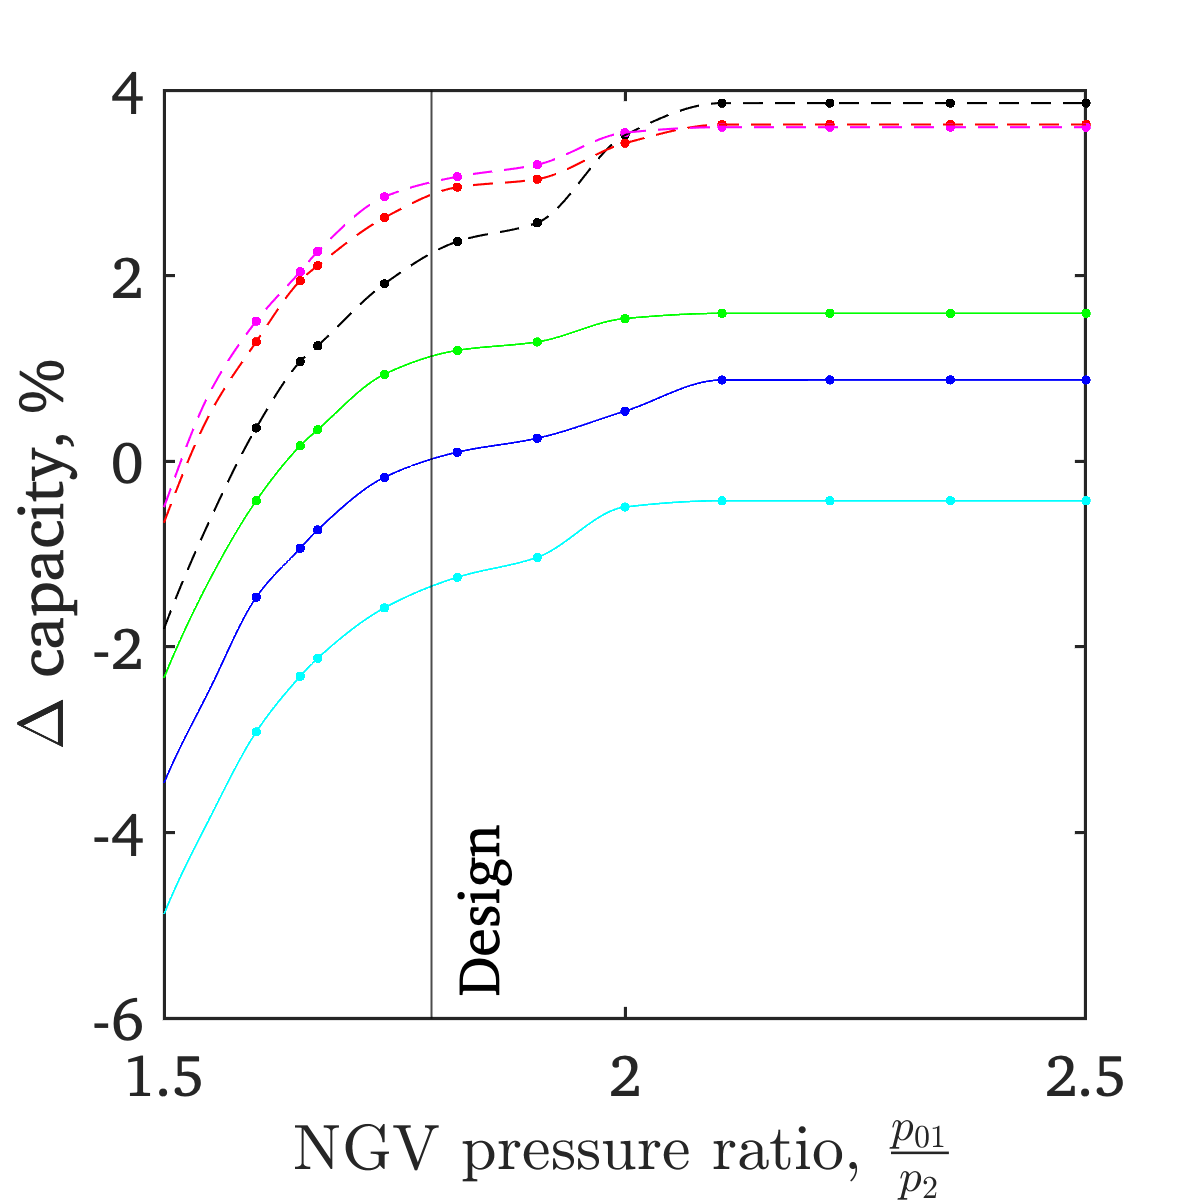
\includegraphics[width=\linewidth]{figs/t900_2d_capacity_trends.png}
	\end{subfigure}
	\begin{subfigure}{.1125\textwidth}
		\centering
		
\includegraphics[width=\linewidth]{figs/t900_2d_capacity_trends_legend.png}
	\end{subfigure}
	\caption{2D capacity trends for 6 Trent 900 NGVs}
	\label{fig:t900_2d_capacity_trends}
\end{figure}

Differences are seen to exist between the capacity trends of the 6 NGVs. Across the range of pressure ratios, all 6 NGVs exhibited a range of approximately 4\% capacity difference. Although the NGVs were all fully choked at the greatest inverse pressure ratio, separate NGVs became choked at significantly different pressure ratios, suggesting that the formation of transonic flow features occured in different locations between the 6 NGVs. The capacity trends are seen to be broadly divided between the M-skew family (K-- serial numbers) and the EP1 family (P-- serial numbers). The 3 M-skew NGVs had comparitively lower flow capacities than the EP1 NGVs at all pressure ratios. The capacities of the EP1 NGVs had comparitively small variation from one another across pressure ratios, but their homogeneity was broken by vane PNS04, which had the lowest flow capacity of the family at low inverse pressure ratio, but switched to have the highest flow capacity at high inverse pressure ratio.

The differing capacity trends may be further discussed by inspecting the shape of the $M=1$ lines formed in the throat regions of the 6 NGVs at a fully choked pressure ratio. These $M=1$ lines are depicted in Figure~\ref{fig:T900_mach1_lines} along with the lines of minimum length between the adjacent NGVs of each standard. 

\begin{figure}[H]
      \centering
      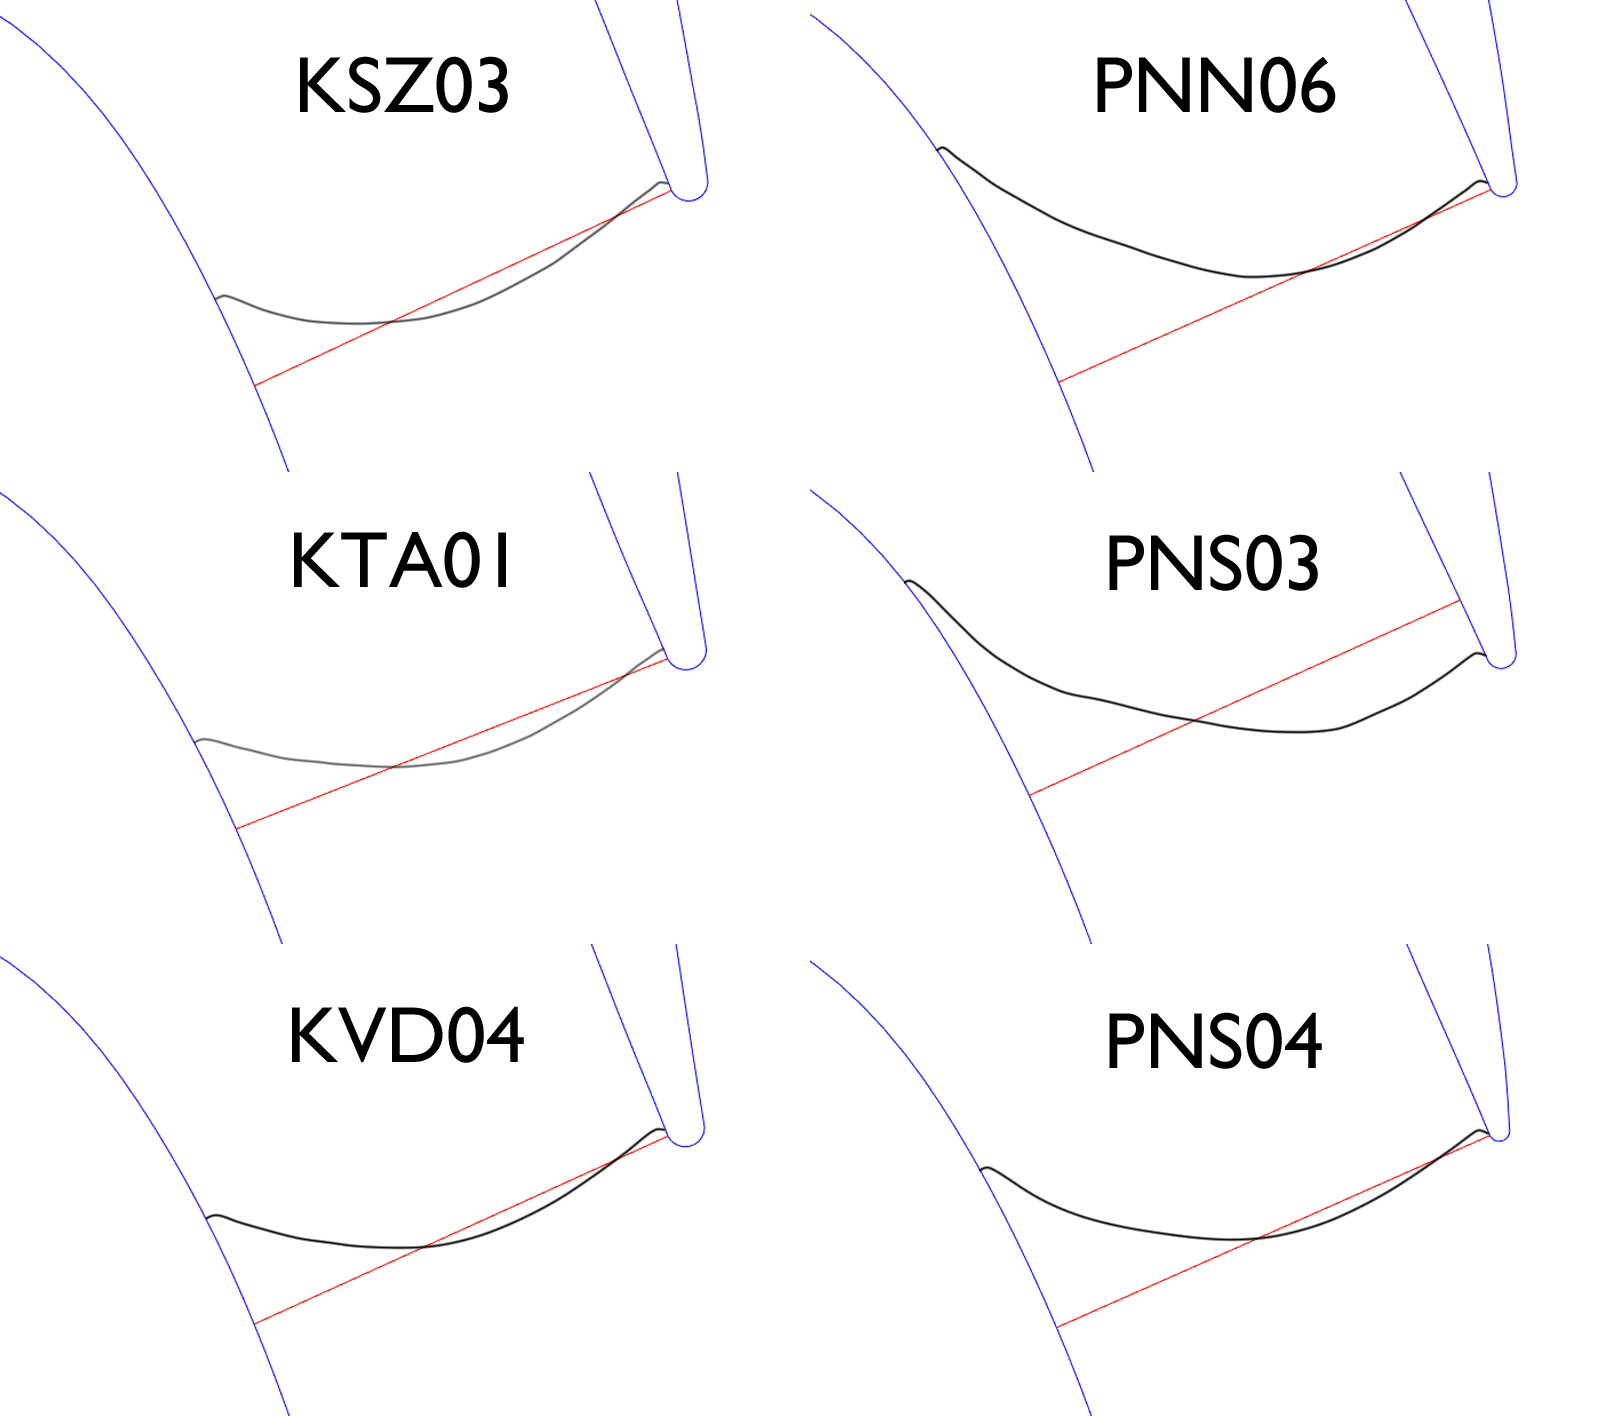
\includegraphics[width=.7\textwidth]{figs/T900_mach1_lines.png}
      \caption{Sonic lines for 6 Trent 900 NGVs}
      \label{fig:T900_mach1_lines}
\end{figure}

In Figure~\ref{fig:T900_mach1_lines}, a trend is visible of the M-skew sonic lines exhibiting smaller deviation from the line of minimum width, compared to the sonic lines of the EP1 NGVs. This suggests that a design choice resulted in a difference in the aerodynamics of the two families of NGV, such that upstream regions of the EP1 flow field reached sonic conditions significantly further upstream of the geometric throat compared to the M-skew flow field. Vane PNS04 presented a significantly different sonic line shape which is taken to correspond to its significantly different capacity trend comapred to the other 2 vanes in its family. It is suggested that its relatively flow-orthogonal sonic line is caused by aerodynamic features that also cause its relatively sudden increase in capacity prior to choking. This cannot be confirmed in the absence of a statistically significant number of NGV geometries to compare.

Discussion is warranted of the relationship between flow capacity and throat area. Consideration is to be made of both throat area in its pure geometric form $A$, and its effective from $A_{eff}$ as defined in equation~\ref{effective_throat_area_integral}. Figure~\ref{fig:T900_2d_capacities_vs_throat_widths} plots the 6 NGVs' variations in capacity at design pressure ratio against their variations in geometric throat width. Both axes are normalised against the largest values in the set. The averages of the M-skew and EP1 families are plotted and lines of gradient 1 are plotted intersecting the average values, such that any deviations from 1-dimensional compressible flow correspond to deviations from the lines of gradient 1.

\begin{figure}[H]
	\centering
	\begin{subfigure}{.45\textwidth}
		\centering
		\includegraphics[width=\linewidth]{figs/T900_2d_capacities_vs_throat_widths.png}
	\end{subfigure}
	\begin{subfigure}{.1125\textwidth}
		\centering
		
\includegraphics[width=\linewidth]{figs/t900_throat_widths_legend.png}
	\end{subfigure}
	\caption{2D NGV capacity percentage delta as a function of 2D throat width for 6 vanes}
      \label{fig:T900_2d_capacities_vs_throat_widths}
\end{figure}

The 6 NGVs are seen to approximately conform to a directly proportional relationship between geometric throat width and flow capacity, suggesting that geometric throat width is a good estimator of flow capacity among NGVs without significant differences in aerodynamic design. The M-skew vanes exhibited notable conformity to this trend. This is in agreement with the observed homogeneity between the M-skew sonic line shapes. It it is suggested that, among the 3 vanes, the 2-dimensional sonic line shapes were scaling linearly with the shape of the geometric throat line, resulting in the observed linear relationship between geometric throat width and flow capacity despite the presence of a 2D flow field. 2D flow features appear to scale proportionately provided the sonic line scales proportionately. In contrast, no correlation was observed between throat area and flow capacity among the EP1 NGVs. Speculation may be limited to the observation that the qualitatively distinct PNS04 vane exhibited significantly lower flow capacity than the other 2 despite having almost identical geometric throat areas.

Although NGV throat width is a good predictor of NGV flow capacity if aerodynamics do not vary significantly, it is not useful if the sonic line is subject to unpredictable changes in shape and location. The resulting heuristic fails to account for the fact that the majority of streamlines within the flow reach sonic conditions at a point other than their point of minimum width. This discrepancy may be investigated by quantifying the effective throat width of each case, instead of the geometric throat area. Matlab was used to implement the integral
\begin{equation}\tag{\ref{effective_throat_area_integral}}
	A_{eff} = 
	\int_{1}^2 \vu*{v} \vdot \vu*{r} dL
\end{equation}
To achieve this, results for $M$ and $x$ and $y$ velocity components were exported from each Fluent solution. These data were imported into Matlab and interpolated onto a structured quaderilateral grid which covered the region around the throat between 2 adjacent NGVs. Within this domain, data points corresponding to the $M=1$ line were identified using an algorithm to detect the cross-over from $M<1$ to $M>1$. A subsequent algorithm was used to order and connect these points into a sonic line. It was then possible to compute the local velocity unit vector $\vu*{v}$ and local unit vector orthogonal to the sonic line $\vu*{r}$ at each point, and to perform the integral. This resulted in Figure~\ref{fig:T900_2d_capacities_vs_effective_throat_widths}, which plots the 6 NGVs' variations in capacity at design pressure ratio against their variations in effective throat width. Both axes are normalised against the largest values in the set. Because the concept of $A_{eff}$ is designed to account for generised variations between NGVs, Figure~\ref{fig:T900_2d_capacities_vs_effective_throat_widths} does not group the NGVs into 2 separate families.

\begin{figure}[H]
	\centering
	\begin{subfigure}{.45\textwidth}
		\centering
		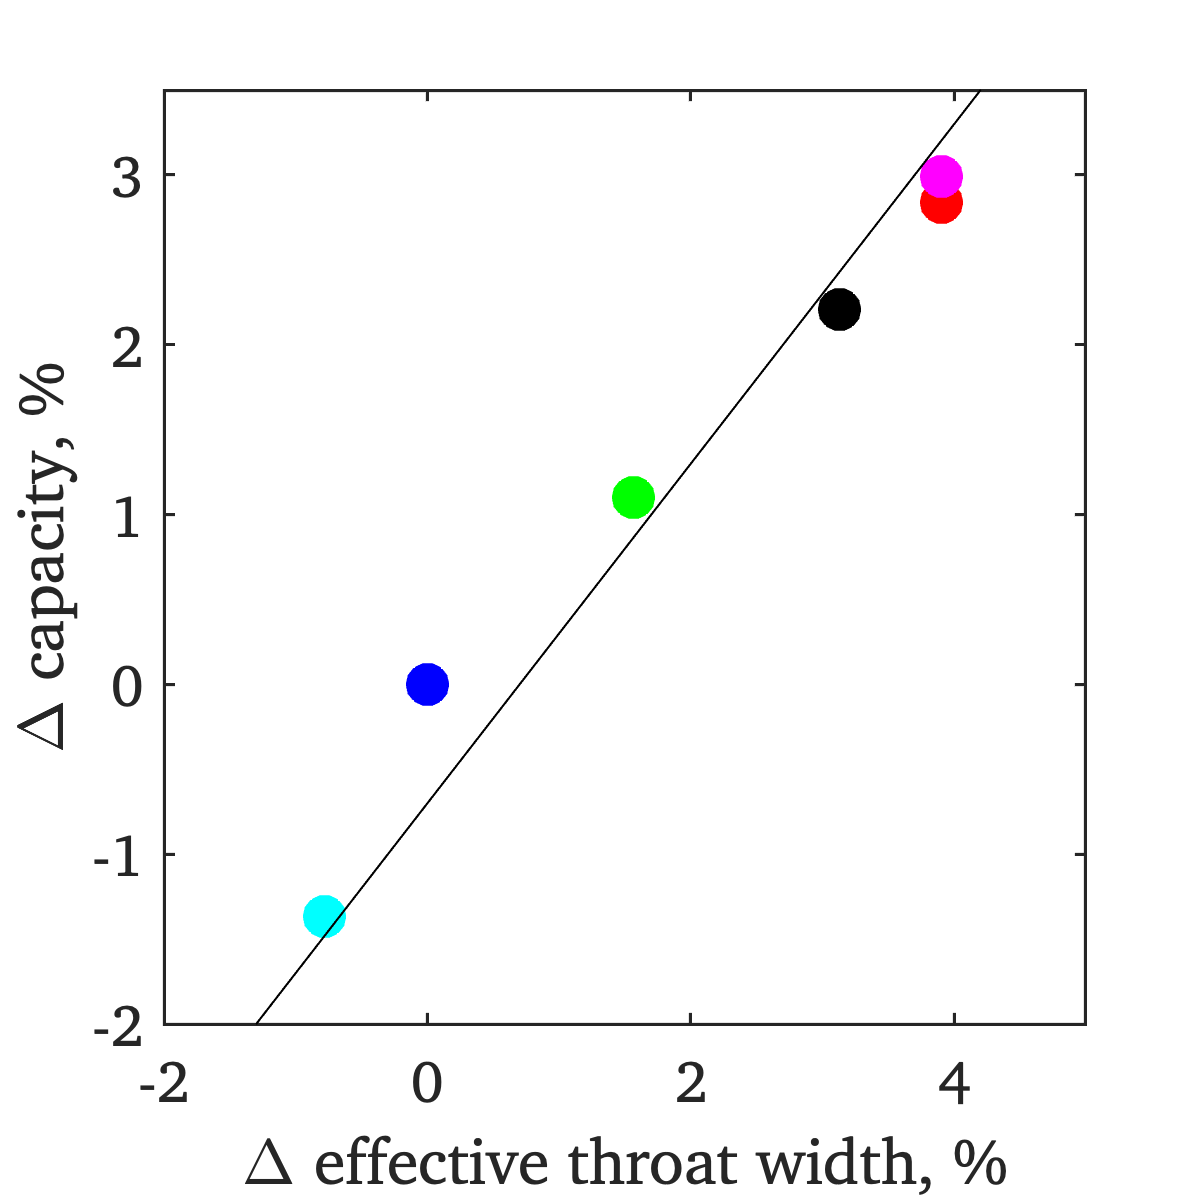
\includegraphics[width=\linewidth]{figs/t900_2d_capacities_vs_effective_throat_widths.png}
	\end{subfigure}
	\begin{subfigure}{.1125\textwidth}
		\centering
		
\includegraphics[width=\linewidth]{figs/t900_2d_capacity_trends_legend.png}
	\end{subfigure}
	\caption{2D NGV capacity percentage delta as a function of 2D $A_{eff}$ for 6 vanes}
      \label{fig:T900_2d_capacities_vs_effective_throat_widths}
\end{figure}

Figure~\ref{fig:T900_2d_capacities_vs_effective_throat_widths} demonstrates the viability of the $A_{eff}$ approach. All six vanes approximately show a directly proportional relationship between flow capacity and effective throat width. This is in agreement with the assumption that the integral definition of $A_{eff}$ amounts to the summation of the 1-dimensional throat widths of every streamline in the flow. However, 3 of the NGVs exhibit significant deviation from direct proportionality, suggesting that the use of the sonic line fails to account for regions of the flow which remain subsonic even at pressure ratios which cause the majority of the flow to choke. The boundary layers are offered as examples of such regions. A possible refinement to the $A_{eff}$ approach may be to combine it with a prediction of the boundary layer thicknesses at the points where the sonic line meets the suction side and pressure side of the NGVs. Heuristics may be devoloped to relate the touch-down points with the predicted boundary layer thicknesses and thus the degree of $A_{eff}$ over-estimation caused by the inclusion of subsonic flow.

$A_{eff}$ remains computable only in the event that a CFD solution has been obtained, by which point flow capacity is already predicted. The next goal is to find an aspect of NGV geometry which can be shown to have a reliable effect on the shape of the $M=1$ line. In this way, the geometric change will have been shown to account for a known change in $A_{eff}$, which has itself been shown to account for known changes in flow capacity in 2 dimensions. Since the M-skew and EP1 families exhibit clear differences in the degree of pre-throat sonic conditions which are present, future studies may examine whether NGVs can be reliably designed to have sonic lines whose shape is predictable. If the sonic line is known by design to be approximately orthogonal to the flow and non-succeptible to fluctuation, it is safe to rely on just 2D geometric throat width to predict variations in NGV flow capacity in 2 dimensions.


\section{2D vs 3D capacity uncertainty}
\label{2d_vs_3d_capacity_uncertainty}

Zamboni defined the Rolls-Royce process for calculating 3D throat area as follows: ``Along each vane span section, the throat line is defined as that line which connects the TE of one vane with the point of minimum distance on the suction surface of the nearby vane in the tangential direction. For a vane with TE slot, the TE point is defined as the start of the cut back... The throat surface interpolates all the throat lines spanwise.'' Their study produced values for throat area of the 6 NGVs in question. These values are listed in Table~\ref{T900_throat_areas}.

\begin{table}[H]
\caption{Throat areas of 6 Trent 900 NGVs}
\label{T900_throat_areas}
\begin{center}
\begin{tabular}{|c|c|c|}
\hline
Production standard & Serial number & Throat area (mm$^2$)\\
\hline
\multirow{3}{*}{M-skewed} & KSZ03 & 1578.4\\
 & KTA01 & 1584.6\\
 & KVD04 & 1571.4\\
 \hline
 \multirow{3}{*}{M EP1} & PNN06 & 1592.0\\
 & PNS03 & 1587.2\\
 & PNS04 & 1598.8\\
\hline
\end{tabular}
\end{center}
\end{table}

The present study compared the 2D data presented in Section~\ref{section_1d_vs_2d_capacity_uncertainty} with Rolls-Royce's 3D CFD predictions of the flow capacities of the same 6 NGVs. The motivation was to analyse the differences between the 2D throat length vs capacity relationship and the 3D throat area vs capacity relationship. The analytical techniqes of Section~\ref{section_1d_vs_2d_capacity_uncertainty} were translated to this 3D relationship where possible.

Figure~\ref{fig:t900_3d_capacity_trends} plots percentage changes in the flow capacity of the 6 NGVs (defined by equation~\ref{capacity_definition} and quantified by the upstream boundary conditions in Table~\ref{T900_parameters}) against inverse pressure ratio $\frac{p_{01}}{p2}$.

\begin{figure}[H]
	\centering
	\begin{subfigure}{.45\textwidth}
		\centering
		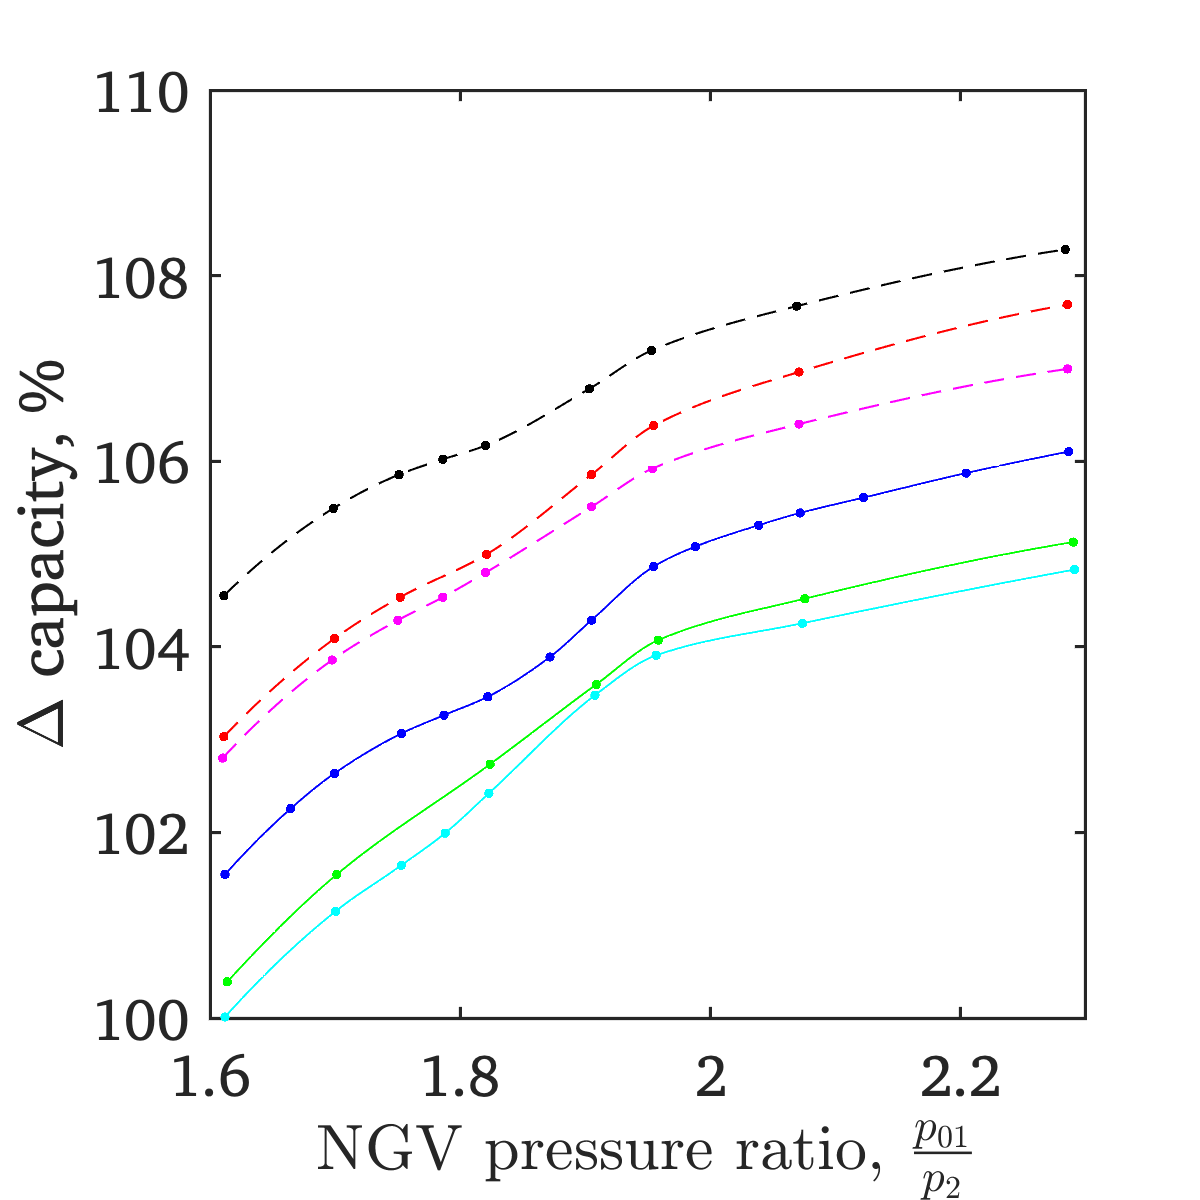
\includegraphics[width=\linewidth]{figs/t900_3d_capacity_trends.png}
	\end{subfigure}
	\begin{subfigure}{.1125\textwidth}
		\centering
		
\includegraphics[width=\linewidth]{figs/t900_2d_capacity_trends_legend.png}
	\end{subfigure}
	\caption{3D capacity trends for 6 Trent 900 NGVs}
	\label{fig:t900_3d_capacity_trends}
\end{figure}

The predominant feature of Figure~\ref{fig:t900_3d_capacity_trends} is that none of the NGVs reaches a choked condition at pressure ratios that resulted in a fully choked condition in the 2D simulations. This suggests that there are significant incursions into the flow from subsonic secondary flows. This alone is sufficient to preclude the present $A_{eff}$ approach in these 3D cases, since it has been shown to be limited even by the presence of thin boundary layers in the 2D cases. In this case, an $M=1$ surface may not exist in a useful sense.

The viability of the geometric throat area approach to 3D data is ilustrated in Figure~\ref{fig:T900_2d_capacities_vs_throat_areas}, which plots the 6 NGVs' variations in capacity at design pressure ratio against their variations in geometric throat area. Both axes are normalised against the largest values in the set. The averages of the M-skew and EP1 families are plotted and lines of gradient 1 are plotted intersecting the average values, such that any deviations from 1-dimensional compressible flow correspond to deviations from the lines of gradient 1.

\begin{figure}[H]
	\centering
	\begin{subfigure}{.45\textwidth}
		\centering
		\includegraphics[width=\linewidth]{figs/T900_3d_capacities_vs_throat_areas.png}
	\end{subfigure}
	\begin{subfigure}{.1125\textwidth}
		\centering
		
\includegraphics[width=\linewidth]{figs/t900_throat_widths_legend.png}
	\end{subfigure}
	\caption{3D NGV capacity percentage delta as a function of 3D throat area for 6 vanes}
      \label{fig:T900_2d_capacities_vs_throat_areas}
\end{figure}

Figure~\ref{fig:T900_2d_capacities_vs_throat_areas} shows that no correlation exists between geometric throat area and flow capacity for the 6 NGVs simulated by Rolls-Royce. This is in agreement with the hypothesis that highly 3-dimensional flow phenomena are present to a degree that predominates over any area-capacity relationship. Future study might divide focus between developing a 3D version of the $A_{eff}$ technique and accessorising it with a model for the subsonic secondary flows that are hypothesised to be present. An overarching goal may be to confirm that secondary flows are indeed the confounding factor that is not captured by 2-dimensional CFD. In any case, motivation is presented to resolve the failure of present analytical techniques in understanding the sensitivity of nozzle guide vane flow capacity to geometric changes.



\chapter{Trailing edge}
\label{chapter_trailing_edge}
%How the trailing edge can drive capacity changes (and loss changes incidentally). These changes are discussed as those happening in-life to the existing engine parts, and also those resulting from an alternative design.
%Why am I including "loss" here, when this part is really about the robustness of capacity predictions on vanes that will change shape with wear? Because the proposed alternative design needs to be decent for loss to be a viable alternative.

%NEEDED DATA:
%-SS cutbacks, all solutions
%-PS cutbacks, all solutions
%-variable cooling rate CFD
%-Larger pictures of the different meshes used
%-Larger contour plots for the different levels of TE SS erosion
%-MinA and M1 lines for the TE SS cutbacks  
%-"Rolls-Royce vs this study" geometry illustration should be remade to be at the same angle as all the flow pictures

%Plan for chapter - answer the following questions:
%1) How does erosion to the SS flange alter 2D mid-span capacity, and which mechanism best explains the changes?
%2) According to the literature, would a 3D investigation into this be justified?
%3) How capacity-predicable would an altrernative design of TE be?
%4) Would said alternative design reduce "loss"?


\section{Effects of trailing edge shape uncertainty on capacity predictability}
\label{effects_of_trailing_edge_uncertainty_on_capacity_predictability}

If nozzle guide vane flow capacity is known to be a function of effective throat area, we must survey the practical reasons for which effective throat area might vary. In a real engine, NGV effective throat area might depart from its design value if the NGVs depart from their design shape, either because of the finite precision of manufacturing, or because of erosion while in service. 

A goal of the present study is to help ascertain how much these off-design conditions might limit the predictability of NGV flow capacity, and to comment on ways to mitigate this limitation. The NGV trailing edge is an area of focus because it is particularly succeptible to both finite-precision and in-service departures from its design shape. 

The trailing edge is succeptible to finite-precision departures from its design shape because of how it is manufactured. Vane pairs are cast to a finite precision as discussed in Section~\ref{section_1d_vs_2d_capacity_uncertainty}, where significant geometric variation appears in vanes even without cooling features. The vanes are then subject to machining to finish off the trailing edge shape. The finishing creates the most aerodynamic trailing edge possible, with a thin suction-side flange that cleanly meets the endwalls, and a flange chord length that is consistent across the span of the trailing edge. The creation of a repeatable minimum geometric area cannot be said to be a primary objective.

The trailing edge is succeptible to in-service departures from its design shape because it is the most fragile part of the vane. The NGV remains largely intact over a lifetime of extremely hot supersonic flow, but the trailing edge flange may be subject to significant erosion. If there is a blockage in any of the plena which feed the trailing edge slot, part of its span will receive reduced coolant flow, accelerating the degradation of the trailing edge flange near that area. Such cooling failures are not uncommon in sandy environments.

This study will consider the potential worst case for in-service erosion of the suction-side flange, namely its complete deletion. This worst-case erosion is assumed to take place at the NGV mid-span because this area is exposed to the greatest flow speeds and temperatures. This justifies 2-dimensional simulation of the mid-span flow. The goal is to parameterise changes to the flange and comment on how these changes alter the effective minimum area and the NGV flow capacity.

2D CFD has been used to model the effects of incremental removal of material from the trailing-edge suction-side flange of an NGV. The baseline geometry is vane KSZ03 from the 6 vanes provided by Rolls-Royce for the work discussed in Chapter~\ref{chapter_geometric_throat_area}. The 2D vane section was produced using the process illustrated in Figure~\ref{fig:2d_geometry_creation}. The overall computational domain was produced as in Figure~\ref{fig:computational_domain_and_boundaries}. Unlike the section of vane KSZ03 studied in Chapter~\ref{chapter_geometric_throat_area}, the NGV trailing edge was not rounded but realistically shaped, and the domain was modified to include a flow inlet within the NGV's trailing edge slot, where inlet mass flow rate was specified. Values for the simulation were set according to Table~\ref{ss_cutbacks_parameters}.

\begin{table}[H]
\caption{Boundary conditions for trailing edge suction-side flange shape uncertainty study}
\label{ss_cutbacks_parameters}
\begin{center}
\begin{tabular}{|c|c|}
\hline
Parameter & Value\\
\hline
NGV series & Rolls-Royce Trent 900\\
NGV turning (degrees) & 76.89\\
Design pressure ratio & 1.79\\
Inlet total pressure (Pa) & $4.33 \times 10^6$\\
Inlet total temperature (K) & 300\\
Outlet static pressure (design) (Pa) & $2.42 \times 10^6$\\
Outlet static temperature (Pa) & 300\\
Coolant mass flow rate & 3\% of mainstream \\
Solver type & Density-based\\
Cell count & 35,000\\
\hline
\end{tabular}
\end{center}
\end{table}

The strategy for geometry alteration and meshing involved dividing the geometry into quadrilateral regions of solid vane that could be sequentially replaced with regions of mesh. Each replacement would incrementally cut back the NGV trailing edge's suction-side flange. This required minor alteration of the trailing edge geometry provided by Rolls-Royce. The curved surface on the inside of the pressure-side lip was changed to a straight line with an angular corner, and the curved tip of the suction-side lip was changed to a square end. Comparison of the shape of manufactured NGVs with the shape of design-intent NGVs demonstrates that the present study's trailing edge treatment is more reflective of the manufactured NGVs, which have corners rather than smooth curves in the places in question. The process of geometry refinement and incremental mesh block creation is illustrated in Figure~\ref{fig:T900_ss_cutbacks_geometry}.

\begin{figure}[H]
      \centering
      \includegraphics[width=.9\textwidth]{figs/T900_ss_cutbacks_geometry.png}
      \caption{Geometry processing scheme for cutbacks to the suction-side flange of a Trent 900 NGV}
      \label{fig:T900_ss_cutbacks_geometry}
\end{figure}

The resulting quadrilateral geometry allowed for the creation of a structured mesh that could be matched with a structured boundary layer mesh of the same design as that depicted in Figure~\ref{fig:t900_mesh_trailing_edge}. Beyond this, an unstructured mesh was created to the same design as that depicted in Figure~\ref{fig:t900_mesh_whole}. Detail of the trailing edge mesh is shown in Figure~\ref{fig:T900_ss_cutbacks_mesh} in a case where the suction-side flange is approximately halfway removed and replaced with structured mesh blocks.

\begin{figure}[H]
      \centering
      \includegraphics[width=.9\textwidth]{figs/T900_ss_cutbacks_mesh.png}
      \caption{Example of mesh for cutbacks to the suction-side flange of a Trent 900 NGV}
      \label{fig:T900_ss_cutbacks_mesh}
\end{figure}

The described mesh, geometry alteration strategy, and boundary conditions were used to perform 11 CFD simulations which incrementally spanned the range of cutbacks between an unaltered trailing edge and a fully removed flange. Solutions were initialised using the solver’s built-in FMG initialisation and Journal scripts as described in Section~\ref{section_1d_vs_2d_capacity_uncertainty}. NGV mass flow rate was saved at each pressure ratio. Full solution data were saved for the final fully choked pressure ratio to enable analysis of the shocks, expansions and M = 1 line at choked conditions. There were 32 increments and typical overall solution times were approximately 10 hours. The SST-kω turbulence model was used.

Figure~\ref{fig:ss_cutbacks_0-3} shows contours of Mach number in the region of the trailing edge for the described study. The depicted range of cutbacks is between the unaltered baseline and the case of $\frac{3}{10}$ removal of the overall length of the trailing edge suction side flange. Inverse pressure ratio is $3.3$, fully choked.

\begin{figure}[H]
	\centering
	\begin{subfigure}{.45\textwidth}
		\centering
		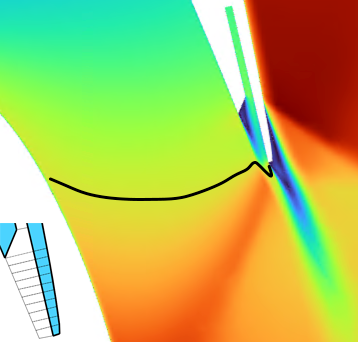
\includegraphics[width=\linewidth]{figs/ss_cutbacks_m1_lines_0.png}
		\caption{Baseline}
		\vspace{0.018\textheight}
	\end{subfigure}
	\hspace{0.05\textwidth}
	\begin{subfigure}{.45\textwidth}
		\centering
		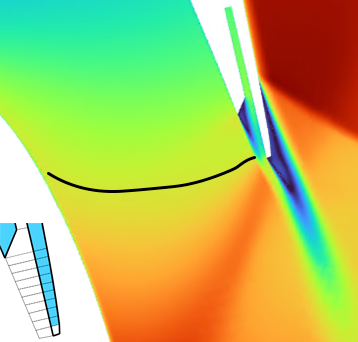
\includegraphics[width=\linewidth]{figs/ss_cutbacks_m1_lines_1.png}
		\caption{$\frac{1}{10}$ cutback}
		\vspace{0.018\textheight}
	\end{subfigure}
	\begin{subfigure}{.45\textwidth}
		\centering
		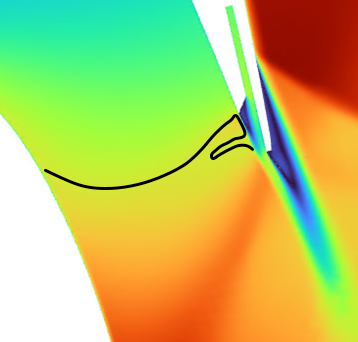
\includegraphics[width=\linewidth]{figs/ss_cutbacks_m1_lines_2.png}
		\caption{$\frac{2}{10}$ cutback}
	\end{subfigure}
	\hspace{0.05\textwidth}
	\begin{subfigure}{.45\textwidth}
		\centering
		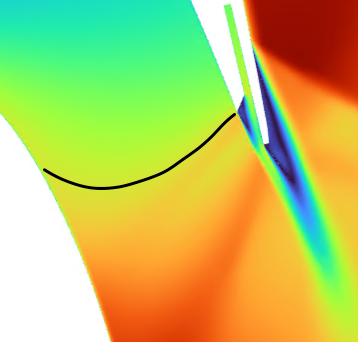
\includegraphics[width=\linewidth]{figs/ss_cutbacks_m1_lines_3.png}
		\caption{$\frac{3}{10}$ cutback}
	\end{subfigure}
	\caption{Effects of small cutbacks on sonic line shape for Trent 900 suction-side flange erosion study}
	\label{fig:ss_cutbacks_0-3}
\end{figure}

Figure~\ref{fig:ss_cutbacks_0-3} illustrates the alteration of the sonic line as the nozzle guide vane's trailing edge suction side flange is incrementally removed until $\frac{3}{10}$ of its length is not present. The sonic line is shown to undergo a fundamental transition over this range of cutbacks, from initially impinging on the trailing tip of the flange in the baseline case, to impinging on the acute corner of the pressure-side flange. The geometric changes are also shown to alter the aerodynamics in the suction-side region upstream of the flange, where an attached shock moved incrementally upstream with progressive cutbacks. Shock-induced boundary layer separation was present, and moved upstream correspondingly with the shock. This resulted in increasingly large separated wake region which was not in alignment with the NGV's turning angle.

Figure~\ref{fig:ss_cutbacks_4-10} shows contours of Mach number in the region of the trailing edge for the described study. The depicted range of cutbacks is between the case of $\frac{4}{10}$ and the case of complete removal of the overall length of the trailing edge suction side flange. Inverse pressure ratio is $3.3$, fully choked.

\begin{figure}[H]
	\centering
	\begin{subfigure}{.45\textwidth}
		\centering
		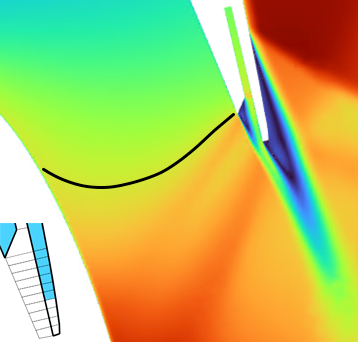
\includegraphics[width=\linewidth]{figs/ss_cutbacks_m1_lines_4.png}
		\caption{$\frac{4}{10}$ cutback}
		\vspace{0.018\textheight}
	\end{subfigure}
	\hspace{0.05\textwidth}
	\begin{subfigure}{.45\textwidth}
		\centering
		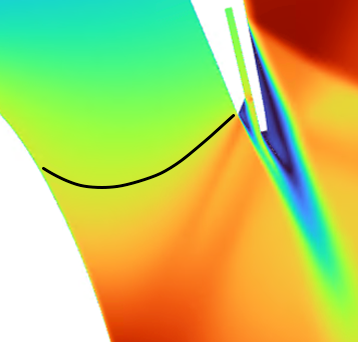
\includegraphics[width=\linewidth]{figs/ss_cutbacks_m1_lines_6.png}
		\caption{$\frac{6}{10}$ cutback}
		\vspace{0.018\textheight}
	\end{subfigure}
	\begin{subfigure}{.45\textwidth}
		\centering
		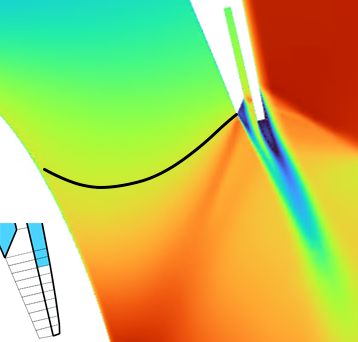
\includegraphics[width=\linewidth]{figs/ss_cutbacks_m1_lines_8.png}
		\caption{$\frac{8}{10}$ cutback}
	\end{subfigure}
	\hspace{0.05\textwidth}
	\begin{subfigure}{.45\textwidth}
		\centering
		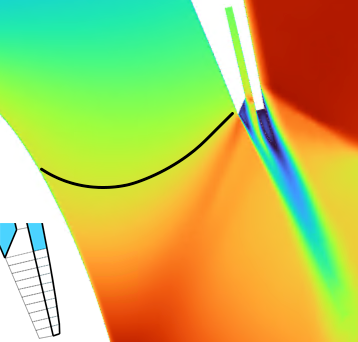
\includegraphics[width=\linewidth]{figs/ss_cutbacks_m1_lines_10.png}
		\caption{Completely cutback}
	\end{subfigure}
	\caption{Effects of large cutbacks on sonic line shape for Trent 900 suction-side flange erosion study}
	\label{fig:ss_cutbacks_4-10}
\end{figure}

Figure~\ref{fig:ss_cutbacks_4-10} illustrates that the shape of the sonic line is not fundamentally altered in the range of $\frac{4}{10}$ to complete removal of the trailing edge suction-side flange. The sonic line is shown to consistently impinge on the acute corner of the pressure-side flange throughout this range of larger cutbacks. Upstream movement of the location of the suction-side attached shock continued to occur. This trend was reversed for the most extreme cases of $\frac{8}{10}$ and complete cutbacks, where the shock transitioned to a downstream location close to the corner of the suction-side flange, resulting in a significantly smaller separated wake region compared to other cases.

The set of Mach number contours and sonic lines suggest that the greatest sensitivity of flow capacity to flange cutbacks is to occur for cutbacks of $\frac{3}{10}$ of the flange or less. The sensitivity of the sonic line shape to the full range of cutbacks is illustrated in Figure~\ref{fig:ss_cutbacks_m1_lines_illustration}. It is further suggested that the location of an attached shock and corresponding boundary layer separation may be sensitive to cutbacks of $\frac{4}{10}$ or more, but this may be imprecisely predicted by the present simulations.

\begin{figure}[H]
      \centering
      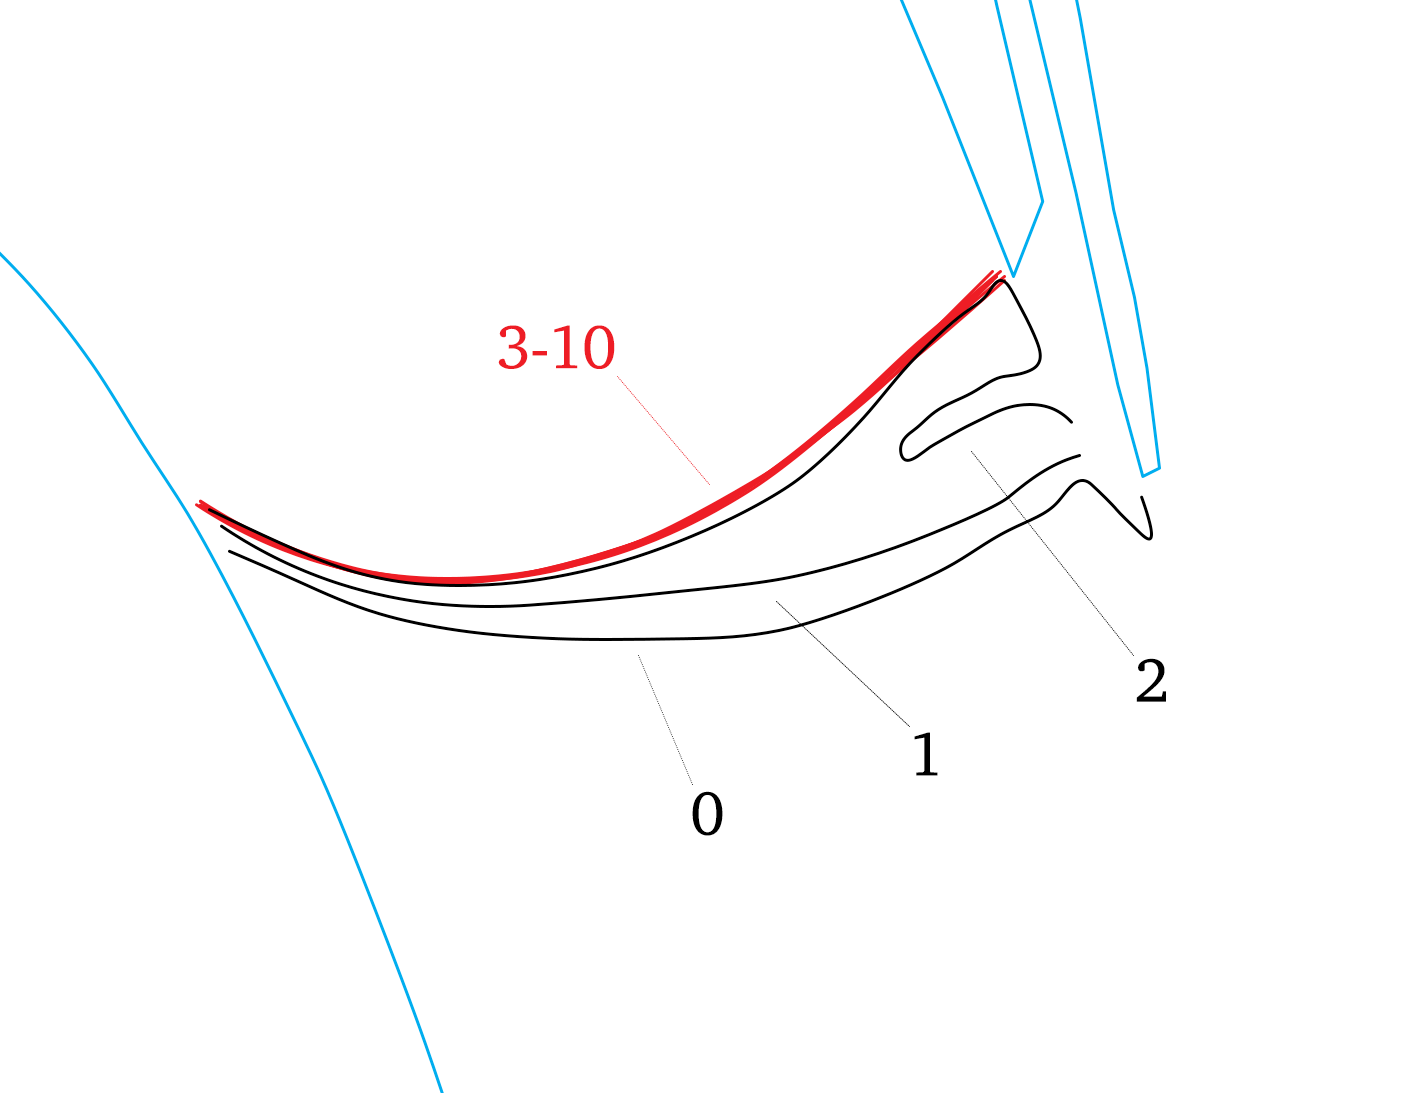
\includegraphics[width=.7\textwidth]{figs/ss_cutbacks_m1_lines_illustration.png}
      \caption{Effects of full range of cutbacks on sonic line shape for Trent 900 suction-side flange erosion study, labelled by $\frac{1}{10}$ of flange size removed}
      \label{fig:ss_cutbacks_m1_lines_illustration}
\end{figure}

Figure~\ref{fig:ss_cutbacks_vs_capacities_pressure_ratios} plots flow capacity change as a function of the amount of the suction-side flange that has been removed. The trend is plotted for 3 inverse pressure ratios: $1.5$, the design value of $1.79$, and a fully choked value of $3.33$.

\begin{figure}[H]
	\centering
	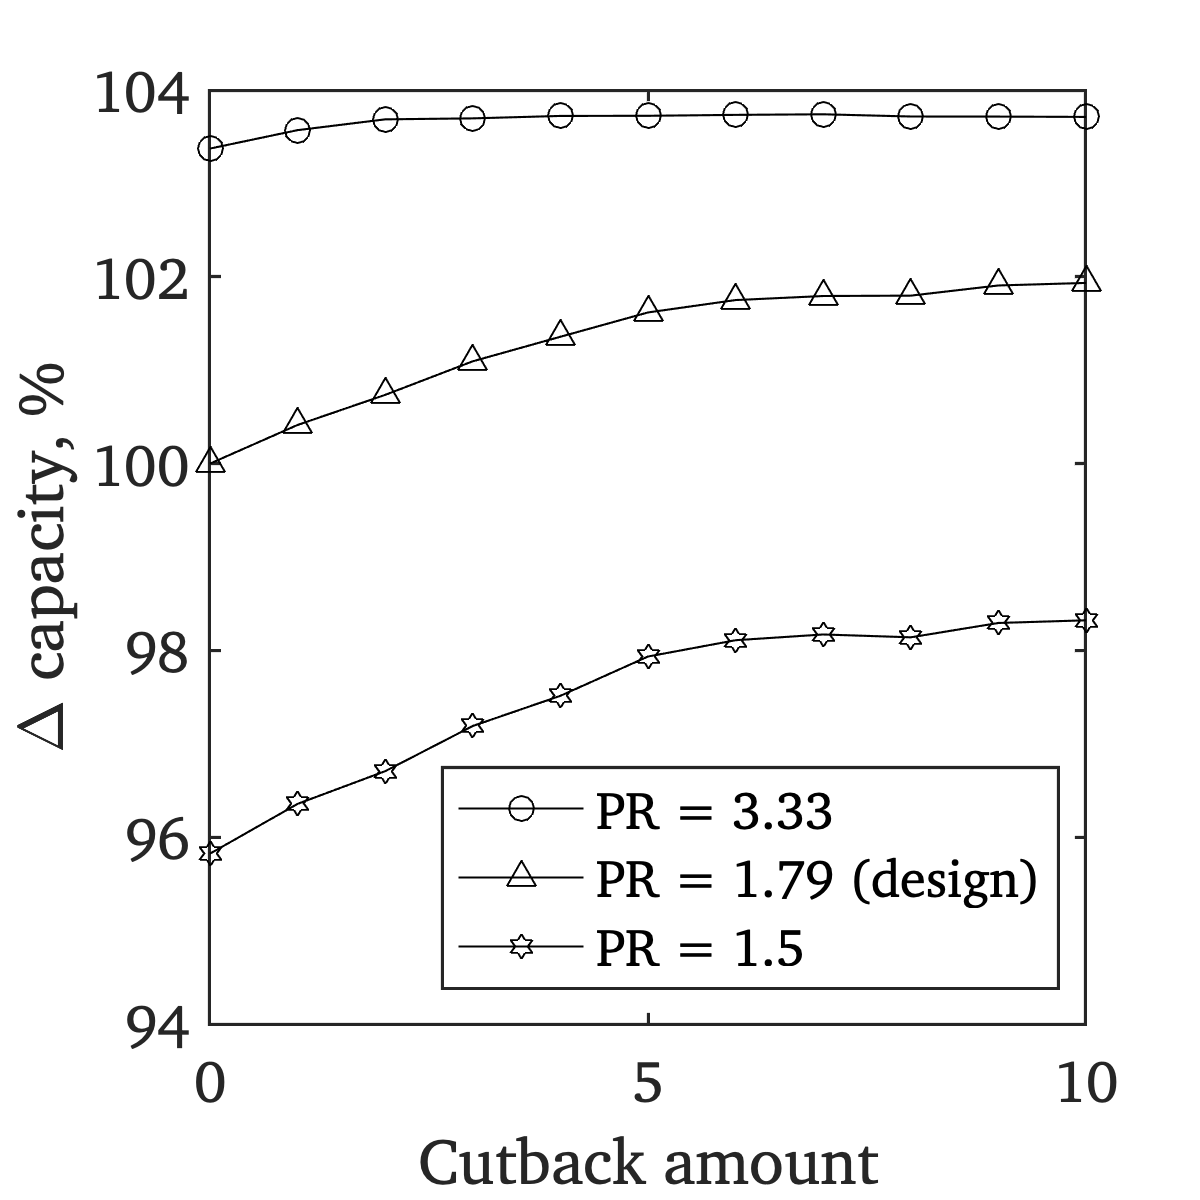
\includegraphics[width=.45\textwidth]{figs/ss_cutbacks_vs_capacities_pressure_ratios.png}
	\caption{2D capacity percentage delta as a function of suction-side flange cutback amount for $3$ pressure ratios}
    \label{fig:ss_cutbacks_vs_capacities_pressure_ratios}
\end{figure}

At an inverse pressure ratio of $3.33$, Figure~\ref{fig:ss_cutbacks_vs_capacities_pressure_ratios} shows a relationship between flow capacity and cutback amount which is in good agreement with the observations made from the corresponding sonic line visualisations. Capacity is shown to be sensitive to cutback amounts of $0$, $\frac{1}{10}$, and $\frac{2}{10}$, and insensitive to cutbacks thereafter. The corresponding sonic lines are observed to vary in shape when capacity varies, and to remain similar in shape when capacity does not vary. The observed switching of the sonic line from the flange-attached mode (at baseline) to the pressure-side-attached mode (at cutbacks of $\frac{3}{10}$ and greater)  is associated with a $0.3$ percentage point increase in capacity. For all cutbacks subsequent to the mode switch, there was no capacity change at this pressure ratio. This is in good agreement with the discussion in Chapter~\ref{chapter_geometric_throat_area} which concluded that the effective throat area of a fully choked nozzle guide vane is predominantly a function of the shape of its sonic line.

At lower inverse pressure ratios for which a sonic line cannot be so analysed, flow capacity varied over a significantly greater range of cutback amounts. This is to be expected by consideration of choked versus non-choked compressible flows. For a fully choked streamline, flow conditions upstream of the sonic line are independent of those downstream. This facilitates the type of approach introduced in Chapter~\ref{chapter_geometric_throat_area}, where the flow conditions immediately upstream of any choked streamline's sonic point are treated as a state of known variables. That streamline's mass flow rate is wholly a function of that state. For a non-choked streamline, its mass flow rate is a function of the state of every point along the streamline, including points downstream of where sonic conditions would appear in choked cases. 

This implies that, in the general case of compressible flow in 2D nozzles, the nozzle flow capacity will increase if the effective passage width is increased at any point along the nozzle. This is in good agreement with the observed relationship between flow capacity and cutback amount at the non-choked pressure ratios. Removal of suction-side flange material increases the effective passage width in the region local to the flange, causing a local decrease in static pressure and increase in dynamic pressure. Because most streamlines are non-choked at the flow region and pressure ratios in question, this state change propagates along the entire streamline with a corresponding increase in mass flow rate.

The maximum change in capacity was $1.9$ percentage points at the design inverse pressure ratio of $1.79$, and $2.5$ percentage points at an inverse pressure ratio of $1.5$. The effect of increasing cutbacks became less pronounced at larger cutback amounts, suggesting that the size of the suction-side flange was ceasing to be the limiting factor on effective passage width for those geometries. Figure~\ref{fig:ss_cutbacks_wakes_design_pr} shows contours of Mach number in the NGV wake region for the full range of cutbacks at the design inverse pressure ratio of $1.79$. 

\begin{figure}[H]
	\centering
	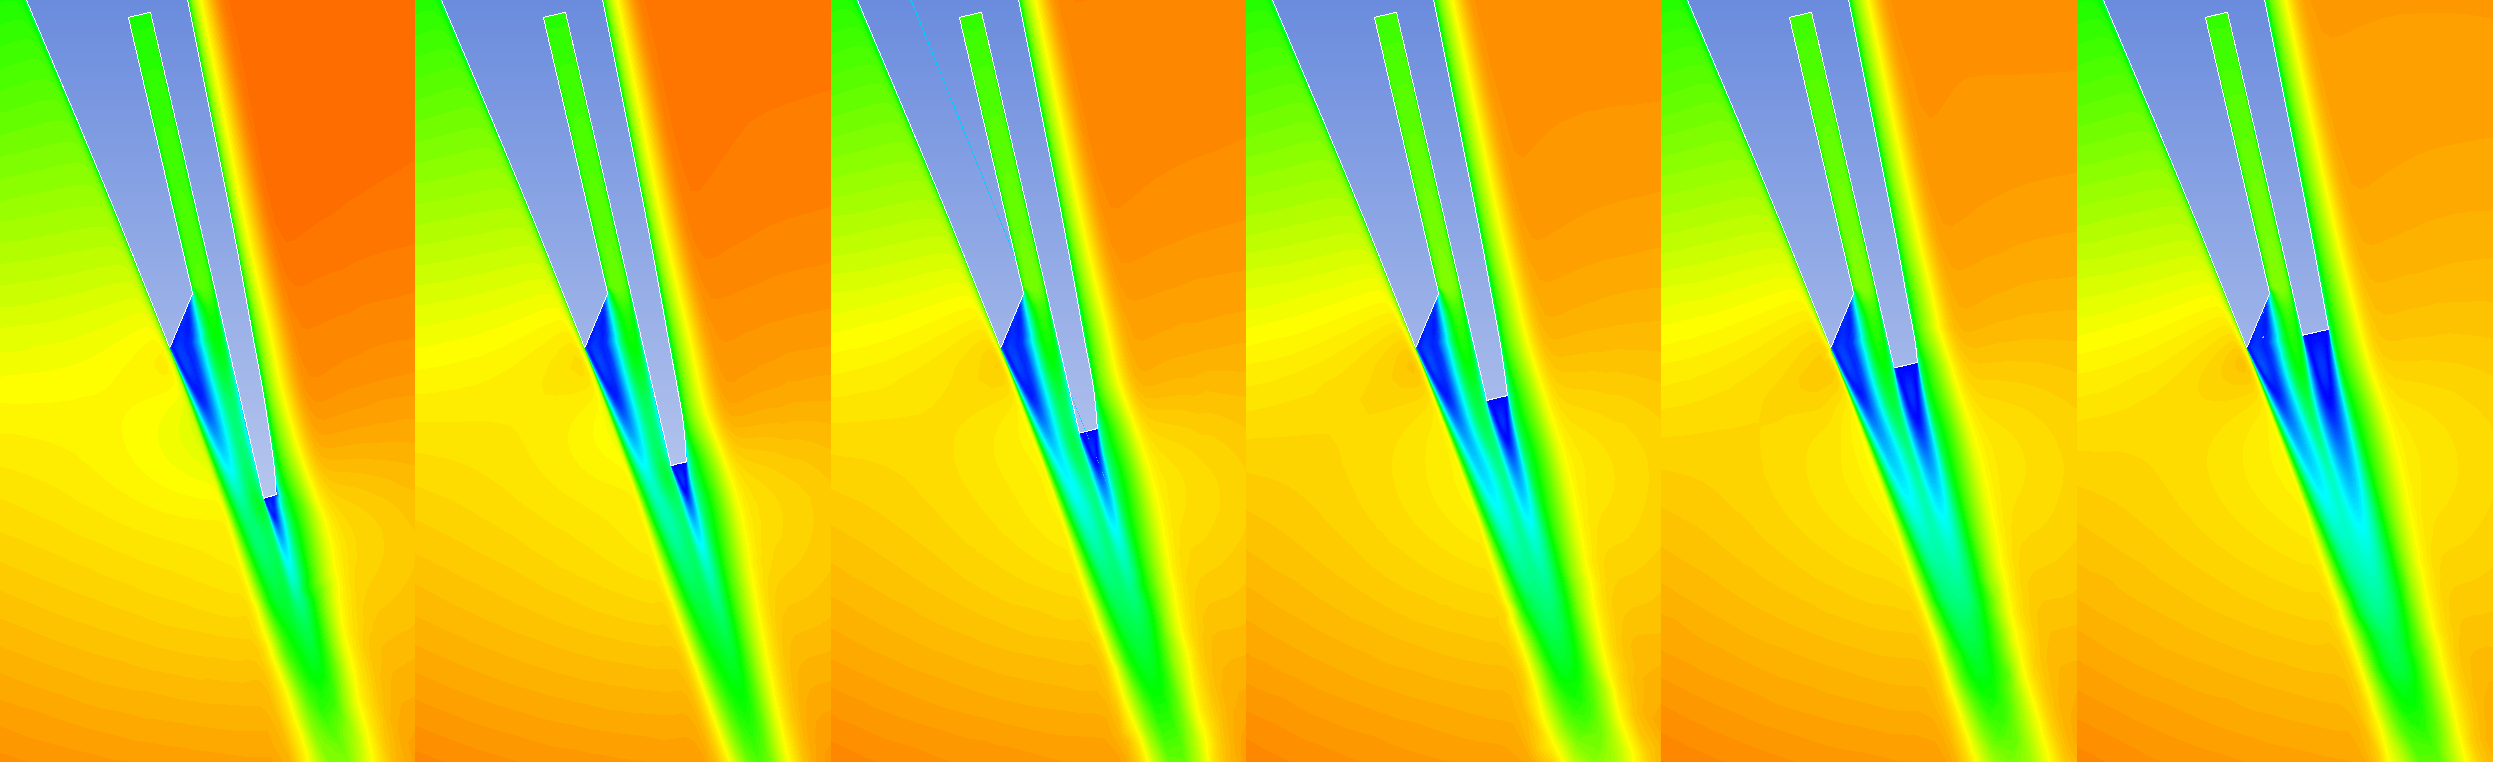
\includegraphics[width=.9\textwidth]{figs/ss_cutbacks_wakes_design_pr.png}
	\caption{Contours of Mach number in the wake region of the Trent 900 suction-side flange erosion study at design inverse pressure ratio of $1.79$}
    \label{fig:ss_cutbacks_wakes_design_pr}
\end{figure}

Key features of Figure~\ref{fig:ss_cutbacks_wakes_design_pr} include an outer wake region (rendered in green) and inner wake regions downstream of the pressure-side lip and suction-side flange (rendered in blue). No fundamental changes occured to the trailing edge's aerodynamics over the range of cutbacks. Mach number is observed to continually increase in the region adjacent to the pressure-side lip, and to continually decrease in the region adjacent to the suction-side flange. The trailing edge aerodynamics were sensitive to geometric changes across the full range of cutbacks. The reduced effect of greater cutbacks on flow capacity may result from two phenomena. Firstly, the local flow acceleration may be limited more by the position of the pressure-side lip than by the suction-side flange at higher cutback values, where the end of the flange is increasingly too far upstream to influence the pressure-side aerodynamics. Secondly, this upstream positioning of the suction-side flange tip is observed to cause a significant increase in outer wake thickness at higher cutback values. This likely reduced the effective passage width in this region and counteracted the predominant effect of flow capacity increasing.

Figure~\ref{fig:ss_cutbacks_vs_capacities_trends} plots trends of flow capacity change versus inverse pressure ratio at each cutback value. The range of inverse pressure ratios includes the design value of $1.79$ but does not extend to fully choked values, which have been shown to be insensitive to cutback amounts greater than $\frac{3}{10}$.

\begin{figure}[H]
	\centering
	\begin{subfigure}{.45\textwidth}
		\centering
		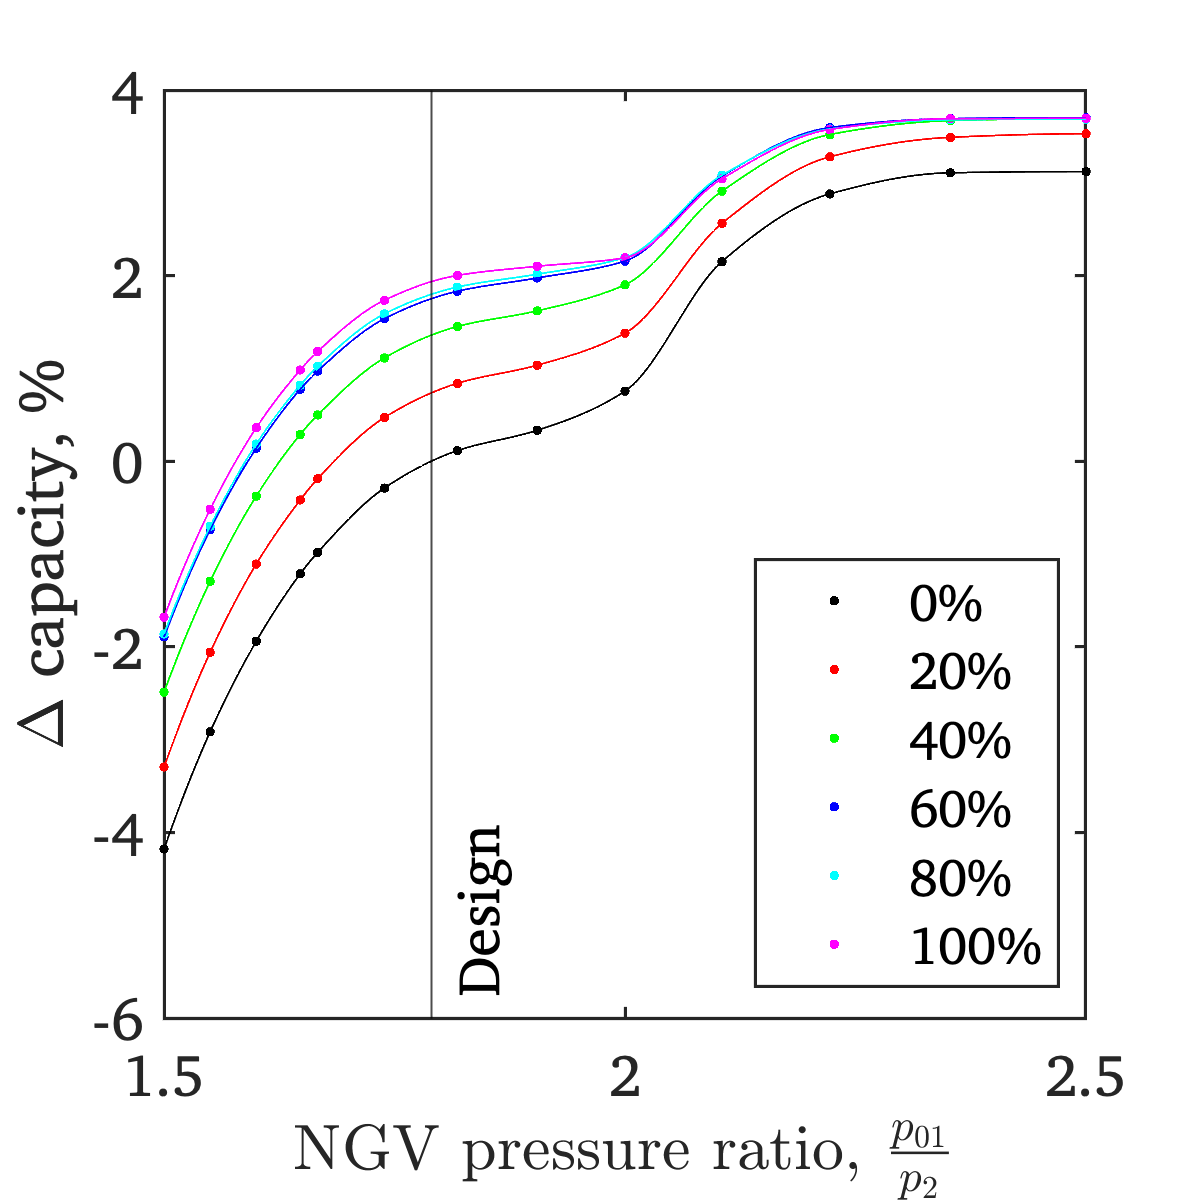
\includegraphics[width=\linewidth]{figs/ss_cutbacks_vs_capacities_trends.png}
	\end{subfigure}
	\begin{subfigure}{.1125\textwidth}
		\centering
		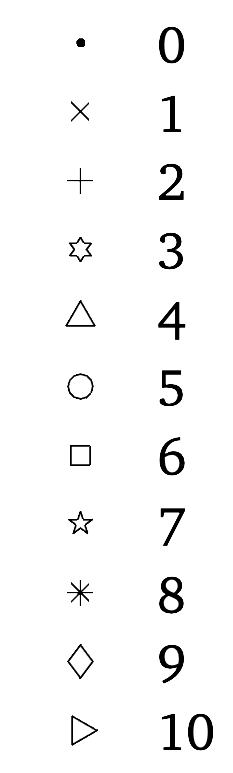
\includegraphics[width=\linewidth]{figs/ss_cutbacks_vs_capacities_trends_legend.png}
	\end{subfigure}
	\caption{2D capacity trends for various suction-side flange cutback amounts}
      \label{fig:ss_cutbacks_vs_capacities_trends}
\end{figure}

In terms of the effects of cutbacks on flow capacity, Figure~\ref{fig:ss_cutbacks_vs_capacities_trends} is in good agreement with Figure~\ref{fig:ss_cutbacks_vs_capacities_pressure_ratios}. The capacity delta produced by full flange removal continuously decreased with increasing inverse pressure ratio, and the capacity trends remained qualitatively similar for all cutback amounts. These observations suggest that the cutback-induced capacity changes and the onset of choking are 2 independent phenomena which do not influence each other. It is conlcuded that, as inverse pressure ratio increased, more streamlines became choked and ceased to be affected by cutbacks downstream of those streamlines' sonic points. It is further concluded that the capacity trend shapes and onsets of choking were unaffected by variable cutbacks, but remained a function of only inverse pressure ratio. This is likely due to the relevant geometric changes taking place downstream of the throat region. This is complementary to the results of Chapter~\ref{chapter_geometric_throat_area}, where geometric changes upstream of the throat resulted in qualitatively distinct capacity trends and dissimilar onsets of choking.


\section{Definitions of loss for trailing edge performance evaluation}
%--How does it perform in terms of loss?
%--First review the literature to decide what is "loss".

Loss may refer to any process whereby the recoverable energy of a turbomachinery flow is reduced during transit through a turbine stage, other than by shaft work, with corresponding entropy creation. Minimisation of loss remains a primary objective of turbomachinery design, but there is not a universal consensus on how to quantify it. As subsequent sections of this thesis will evaluate the losses caused by changes to the trailing edge of nozzle guide vanes, the purpose of this section is to review various definitions of loss from the literature and to facilitate the use of appropriate definitions in the present study.

Daniel Back da Trinidade et al~\cite{trinidade_loss} characterised sources of loss as shock loss, profile losses, tip leakage, endwall losses, and cooling losses. Tip leakage results from flow through the clearance space between the vane tips and the casing. It will not be considered by the present study, since the present study is of fixed NGVs. Endwall losses result from 3-dimensional secondary flows, and will not be considered in the present study which is of 2-dimensional phenomena.

Trinidade et al characterised shock loss as resulting from entropy creation across the shock wave during supersonic flow. The present study will consider this mechanism during discussion of CFD results at choking pressure ratios.

Profile loss was characterised by entropy creation by viscosity in the boundary layer on the blade surface. Entropy generated near the blade's trailing edge was considered as profile loss due to the high entropy creation in the wake region following flow separation at the trailing edge. The authors extended this definition to include the entropy generated as the flow turns tightly around the trailing edge curvature and forms expansion waves.

The authors also defined the category of cooling losses to refer to the aerodynamic penalties incurred by cooling in general, namely ``thicker blade profiles from coolant holes, interaction of coolant film with the blade boundary layer, mixing losses between coolant and main flow and endwall losses.'' The present study seeks to isolate the mechanisms whereby film cooling causes boundary layer changes and mixing effects, discussing film cooling in Chapter~\ref{chapter_leading_edge}.

The present study seeks to define a coefficient of NGV total pressure loss whose arguments are flow measurements or numerically predicted parameters. It is first useful to consider the motivation for quantifying loss in terms of total pressure. This approach treats the nozzle guide vane problem analagously to the problem of flow in a rough pipe, where frictional forces must be balanced by a negative total pressure gradient in the downstream direction. The greater the sum of frictional forces, the greater the loss of total pressure between the inlet and outlet. Total pressure loss can thus aggregate all aerodynamic drag forces acting on the nozzle guide vane or other component.

In an experimental or computational domain, the total pressure loss between inlet and outlet is $p_{01} - p_{02}$. It is intuitive to normalise this against the upstream total pressure $p_{01}$ but it is more useful to normalise it against $p_{01} - p_2$, where $p_2$ is the outlet static pressure. $p_{02}$ never assumes a value greater than $p_{01}$ or less than $p_2$, so if a total pressure loss coefficient is quantified as
\begin{equation}\label{total_pressure_loss_coefficient}
C_{pt} = \frac{
p_{01} - p_{02}
}{
p_{01} - p_2
}
\end{equation}
then the coefficient will be $0$ in the case of no total pressure loss, and $1$ in the extreme case of $p_{02} = p_2$.

Paul W. Giel et al~\cite{giel_te_thickness}, whose findings will be discussed in Section~\ref{performance_of_an_alternative_trailing_edge_design}, surveyed the total pressure wake profiles of a blade at mid-span. They defined a total pressure loss coefficient as in equation~\ref{total_pressure_loss_coefficient}, where $p_{01}$ and $p_{02}$ were the inlet and wake total pressures, and $p_2$ was the wake static pressure. 

Jie Gao et al~\cite{gao_te}, whose findings will be discussed in section~\ref{effects_of_trailing_edge_uncertainty_on_capacity_predictability}, defined a total pressure loss coefficient as
\begin{equation}
{}_{Gao}C_{pt} = \frac{
p_{01} - p_{02}
}{
p_{02} - p_2
}
\end{equation}

This definition is equivalent to normalising the total pressure loss against the downstream dynamic pressure. In the case of simulations where the boundary conditions $p_{01}$ and $p_2$ are set, NGV geometry is the independent variable and $p_{02}$ is the dependent variable. It is thus less convenient for the present study to use Gao et al's loss coefficient formulation, since it does not scale linearly across a range of $p_{02}$. The definition in equation~\ref{total_pressure_loss_coefficient} will be used for this reason.

Where subsequent sections are to compare the findings of Giel et al, Gao et al, and other studies of loss, it is required to formulate the total pressure loss coeffient consistently. Gao's definition of $C_{pt}$ may be expanded by Taylor series on the constant $p_{01}$ and as a function of $p_{02}$ as
\begin{equation}
f\left(p_{02}\right) = \\
f\left(p_{01}\right) +
f'\left(p_{01}\right) \left(p_{02} - p_{01}\right) +
\frac{1}{2!} f''\left(p_{01}\right) \left(p_{02} - p_{01}\right)^2 +
...
\end{equation}
where $f^n\left(p_{01}\right)$ may be shown by differentiation to be
\begin{equation}
f^n\left(p_{01}\right) =
\frac{
	\left(-1\right)^n n !
}{
	(p_{01} - p_2)^n
}
\end{equation}
This results in the following mappings between the two definitions of total pressure loss coefficient.
\begin{equation}
{}_{Gao}C_{pt} = 
\sum_{n=1}^{\infty}
C_{pt}^n
\end{equation}
\begin{equation}
C_{pt} = 
\sum_{n=1}^{\infty}
\left(-1\right)^{n-1}
{}_{Gao}C_{pt}^n
\end{equation}

Since the total pressure loss coefficient quantifies loss as a summation of all drag forces on the NGV, loss may also be quantified as the total amount of kinetic energy dissipated between inlet and outlet, of the form
\begin{equation}\label{ke_loss_form}
\zeta =
\frac{KE_1 - KE_2}{KE_1}
=
1 - \frac{KE_2}{KE_1}
\end{equation}

Kinetic energy may be formulated using the compressible form of Bernouilli's equation as
\begin{equation}\tag{\ref{compressible_bernouilli}}
v = 
\sqrt[•]{ 
2 \left( \frac{\gamma}{\gamma - 1} \right) \left[ \frac{p_0}{\rho_0} - \frac{p}{\rho} \right] 
}
\end{equation}
\begin{equation}
v =
\sqrt[•]{ 
	2 \left( \frac{\gamma}{\gamma - 1} \right)
	R T_0
	\left[
		1 - \left(
			\frac{p_0}{p}
		\right)
		^\frac{1-\gamma}{\gamma}
	\right] 
}
\end{equation}
The flow's kinetic energy at a given station is thus of the form
\begin{equation}
KE(p) \sim
1 - \left(
	\frac{p_0}{p}
\right)
^\frac{1-\gamma}{\gamma}
\end{equation}
allowing equation~\ref{ke_loss_form} to be written as
\begin{equation}
\zeta = 
1 - 
\frac{
	1 -
	\left(
		\frac{p_{02}}{p_2}
	\right)
	^\frac{1-\gamma}{\gamma}
}{
	1 -
	\left(
		\frac{p_{01}}{p_2}
	\right)
	^\frac{1-\gamma}{\gamma}
}
\end{equation}
\begin{equation}\label{ke_loss_definition}
\zeta = 
\frac{ 
	\left(
		\frac{p_{01}}{p_{02}}
	\right)
	^\frac{\gamma-1}{ \gamma } - 1 
}{
	\left(
	\frac{p_{01}}{p_{2}}
	\right)
	^\frac{\gamma-1}{ \gamma } - 1 
}
\end{equation}
This definition of kinetic energy loss coefficient was used by Giel et al. Like the total pressure loss coefficient, it takes a value of $0$ in the case of no loss where $p_{02} = p_{01}$, and $1$ in the extreme case of $p_{02} = p_2$.

Ranjan Saha et al~\cite{saha_loss} experimentally investigated the loss effects of shower-head and trailing edge cooling in an annular sector. By defining kinetic energy loss in 3 alternative ways, the authors demonstrated the extent to which computed loss can vary depending on definition. Discrepancies were shown to result from how the coolant kinetic energy is accounted for. Where the ratio of coolant mass flow rate to mainstream mass flow rate was $Y$, the authors defined kinetic energy loss as
\begin{equation}\label{saha_loss_definition}
\zeta = 
1 -
\frac{ 
	\left( 1 + Y \right) 
	\left(
		1 -
		\left(
			\frac{p_2}{p_{02}}
		\right)
		^\frac{\gamma-1}{\gamma}
	\right)
}{
	\left(
		1 -
		\left(
			\frac{p_2}{p_{01}}
		\right)
		^\frac{\gamma-1}{\gamma}
	\right)
	+Y
	\left(
		1 -
		\left(
			\frac{p_2}{p_{0c}}
		\right)
		^\frac{\gamma-1}{\gamma}
	\right)
}
\end{equation}
In the case of no coolant flow ($Y=0$) this is equivalent to the definition in equation~\ref{ke_loss_definition}. Equation~\ref{saha_loss_definition} is equivalent to the loss definition defined by Mathias Deckers and John D. Denton~\cite{deckers_loss} in the case of no significant temperature difference between coolant and mainstream, as in a significant proportion of experimental studies.

Where coolant flow is present, equation~\ref{saha_loss_definition} requires a local value of $Y$ in order to obtain the loss at any particular point. Assuming that the coolant concentration is a function of the local total pressure loss compared to an uncooled vane, the authors redefined $Y$ as a function of spanwise distance $x$ as
\begin{equation}
\frac{Y\left(x\right)}{Y_{max}}
=
\frac{
	p_{02uc} - p_{02}\left(x\right)
}{
	\left| p_{02uc} - p_{02} \right|_{max}
}
\end{equation}
where $p_{02uc}$ was the total pressure downstream of the cascade with no cooling, $p_{02}$ was the total pressure downstream of the cascade as a function of spanwise distance (with cooling), and $\left[ p_{02uc} - p_{02} \right]_{max}$ denotes the maximum possible difference in downstream total pressure between the uncooled and the cooled cases. Reasoning that this total pressure difference is maximal when $p_{02}=p_{01}$ and $p_{02}=p_{wake}$ (the total pressure in the wake region), Saha et al thus defined their function for local coolant/mainstream mass flux ratio as
\begin{equation}
\frac{Y\left(x\right)}{Y}
=
\frac{
	p_{02uc} - p_{02}\left(x\right)
}{
	p_1 - p_{02wake}
}
\end{equation}
By substituting this definition of $Y$ into equation~\ref{saha_loss_definition}, Saha et al arrived at their novel definition of kinetic energy loss intended to solve the problem of unphysical loss in the free-stream where the previous definition erroneously assumed the presence of coolant. Their new definition is able to use the nominal values for shower-head and trailing edge coolant mass flow ratio and adjust the coolant profile according to the aforementioned function of spanwise distance. Using measurements from a downstream traverse in their linear cascade, the novel loss definition was found to produce loss profiles that were in good agreement with equation~\ref{ke_loss_definition} and in disagreement with equation~\ref{saha_loss_definition}.
		
		
\begin{comment}
\section{Performance of an alternative trailing edge design}
\label{performance_of_an_alternative_trailing_edge_design}
%--Centred-ejection option (PS cutbacks) (and could it reduce loss) and what happens as its geometry is changed to gradually look more like an existing design
%--We must also consider broader TE manufacturing changes that are likely to happen on purpose - the switch to CMC manufacturing of turbine blades. How will this change the game, and what tolerances are expected?

Improved materials and manufacturing techniques may neccessitate alternative trailing edge geometries. Paul W. Giel et al~\cite{giel_te_thickness} noted that ``in the pursuit of higher turbine inlet temperatures for reduced fuel burn and emissions consistent with NASA's goals~\cite{giel_nasa_reference}, Ceramic Matrix Composite (CMC) materials are now being implemented in gas turbine engines...They enable higher turbine inlet temperatures, thus enabling higher overall pressure ratios (OPRs) for the engine and higher thermal efficiency.'' 

The authors used a linear cascade to measure the aerodynamic performance of a set of blades representing the geometric constraints of the CMC manufacturing method. Of main concern was the constraint that ``the trailing edge thicknesses of CMC blades are anticipated to be significantly larger than those of current state-of-the-art metallic blades,'' which may be expected to cause increased loss. 

\textcolor{red}{Discuss other justifications for studying this design - is it more predictable because it suffers less erosion?}

\textcolor{red}{Introduce my alternative design: 2D CFD was done on an alternative design of TE featuring centred coolant ejection. This shape of TE was also incrementally cut back on the pressure side so as to more resemble the existing TE design.}

\textcolor{red}{Present boundary conditions.}

\begin{table}[H]
\caption{Boundary conditions for trailing edge centred-ejection design study}
\label{ps_cutbacks_parameters}
\begin{center}
\begin{tabular}{|c|c|}
\hline
Parameter & Value\\
\hline
NGV series & Rolls-Royce Trent 900\\
NGV turning (degrees) & 76.89\\
Design pressure ratio & 1.79\\
Inlet total pressure (Pa) & $4.33 \times 10^6$\\
Inlet total temperature (K) & 300\\
Outlet static pressure (design) (Pa) & $2.42 \times 10^6$\\
Outlet static temperature (Pa) & 300\\
Solver type & Density-based\\
Cell count & 35,000\\
\hline
\end{tabular}
\end{center}
\end{table}

\textcolor{red}{Present mesh with larger and better pictures, and show how the mesh is altered as the design is altered.}

\textcolor{red}{Plot capacity trends for the centred-ejection designs vs the baseline.}

\textcolor{red}{Is there better capacity predictability because the effects of erosion are less pronounced due to the thicker flanges?}

\textcolor{red}{Discuss whether this loss may be worse or better if a centred-ejection design is used, still perhaps plotting more than one definition of loss.}

\textcolor{red}{When using this configuration, is there an optimal blowing rate that might re-energise the base region? Plot blowing rate vs loss, remembering that the graph I currently have is erroneously for the other type of TE, not for the centred-ejection kind. Should I try to re-run just this one thing?}

\textcolor{red}{Compare my centred-ejection TE with a "naturally-formed by erosion" centred-ejection TE from the literature.} 


A blowing rate study:

\textcolor{red}{Jie Gao - Experimental and numerical investigations of trailing edge injection in a transonic turbine cascade~\cite{gao_te}}
	\textcolor{red}{Arguing: TE coolant ejection is good for reducing the wake size and reducing shock effects on the exit angle}
	\textcolor{red}{Raw data: Their experimental and CFD linear cascade, five-hole probe data and surface pressure plots, downstream loss profile}
	\textcolor{red}{I discuss: Does it match my blowing rate study? Do my turning angles agree with theirs as Mach number changes? Do I see the same reduction of shocks? Do I broadly agree about the benefits of TE ejection? Remember badly-predicted turning angles are like bad capacity predictions}
	\textcolor{red}{I also cite: Whoever's loss definition they use - why didn't they compare it to others?}
	\textcolor{red}{My raw data: A lot of my own TE CFD}
	
Gao et al experimentally and numerically investigated the external flow field near the trailing edge of a linear cascade with trailing edge injection. The authors' focus was on the effects of the trailing edge coolant flow on the vane's loss mechanisms and flow exit angle. Without trailing edge injection, increased exit isentropic Mach number caused the appearance of trailing edge suction side shock waves which altered the flow angle. With trailing edge injection, there was a slight reduction in this shock effect but a strong reduction in the shock wave near the trailing edge pressure side.

\end{comment}



\chapter{Leading edge}
\label{chapter_leading_edge}
%How the LE matters too.

%NEEDED DATA:
%-XWB 84K SS cooling hole 2D CFD solutions - not sure if there are multiple PRs converged, can we check that?
%-XWB 84K SS cooling hole quasi-3D solutions - again not sure about other PRs
%-More detailed and extensive surface pressure plots of the XWB CFD
%-Surveys of total and static pressure across the passage at or shortly before the throat, to see how it changes with the hole moving
%-Plot of how coolant TP compares to mainstream TP at each different injection point - this could all be compared to Hambidge's analytical work on capacitty and coolant ejection
%-More illustative contour plots showing any differences between the two turbulence models

%Plan for chapter - answer the following questions:
%1) How is capacity affected by where exactly additional film coolant is introduced?
%2) What current models best explain the effects of film coolant row location on capacity?
%3) What corrections are necessary to interpret these 2D slot results in the real context of 2 rows of holes?

\textcolor{red}{It is sometimes necessary to add extra cooling holes on the suction-side at the LE.}

\textcolor{red}{Coolant introduced into this part of the flow has complex interactions with the mainstream, affecting NGV capacity.}
 
 
\section{sensitivity of capacity to cooling holes on the leading suction side}

\textcolor{red}{Adding cooling holes causes complex effects - here discussed as loss, so I need citations for capacity too:}
\textcolor{red}{Jie Gao - Experimental and numerical investigations of hole injection on the suction side throat of transonic turbine vanes in a cascade with trailing edge injection~\cite{gao_te_and_film_cooling}}
		\textcolor{red}{Arguing: Like their above paper but with a SS cooling slot. It causes passage blockage, a thicker wake, and more loss. But when there are shock waves, the film coolant enhances the TE PS shock but reduces the TE SS shock, which could be used toreatly reduce the TE SS shock if the injection is upstream of the throat}
		\textcolor{red}{Raw data: Their experimental and CFD linear cascade, with strong emphasis placed on the loss definitions and techniques established by Denton and Xu, Mee et al, and Schobieri}
		\textcolor{red}{I discuss: Ways in which my SS injection might interact with the flow (including shockwaves) as they suggest. Will I see it without having TE injection too?}
		\textcolor{red}{I also cite: Denton and Xu, Mee et al, and Schobieri for established precident on loss quantification}
		\textcolor{red}{My raw data: My moving coolant row study}

\textcolor{red}{2D CFD was done on an XWB NGV with no coolant features apart from the addition of a single cooling row on the upstream suction side. The position of this featrure was varied, thus varying whereabouts in the flow the coolant was introduced.}

\textcolor{red}{Present boundary conditions.}
\begin{table}[H]
\caption{Boundary conditions for suction-side cooling hole position study}
\label{SCH_parameters}
\begin{center}
\begin{tabular}{|c|c|}
\hline
Parameter & Value\\
\hline
NGV series & Rolls-Royce Trent XWB 84K\\
NGV turning (degrees) & $73.97$\\
NGV throat width (m) & $1.25 \times 10^-2$\\
Design pressure ratio & $1.65$\\
Inlet total pressure (Pa) & $4.33 \times 10^6$\\
Inlet total temperature (K) & $300$\\
Outlet static pressure (Pa) & $2.63 \times 10^6$\\
Outlet static temperature (Pa) & $300$\\
Coolant/mainstream mass flow ratio & $0.003$\\
Solver type & Density-based\\
Cell count & $40,000$\\
\hline
\end{tabular}
\end{center}
\end{table}

\textcolor{red}{Present mesh, showing how the variable location coolant row is introduced.}
\begin{figure}[H]
  \centering
  \begin{subfigure}{.9\textwidth}
    \centering
    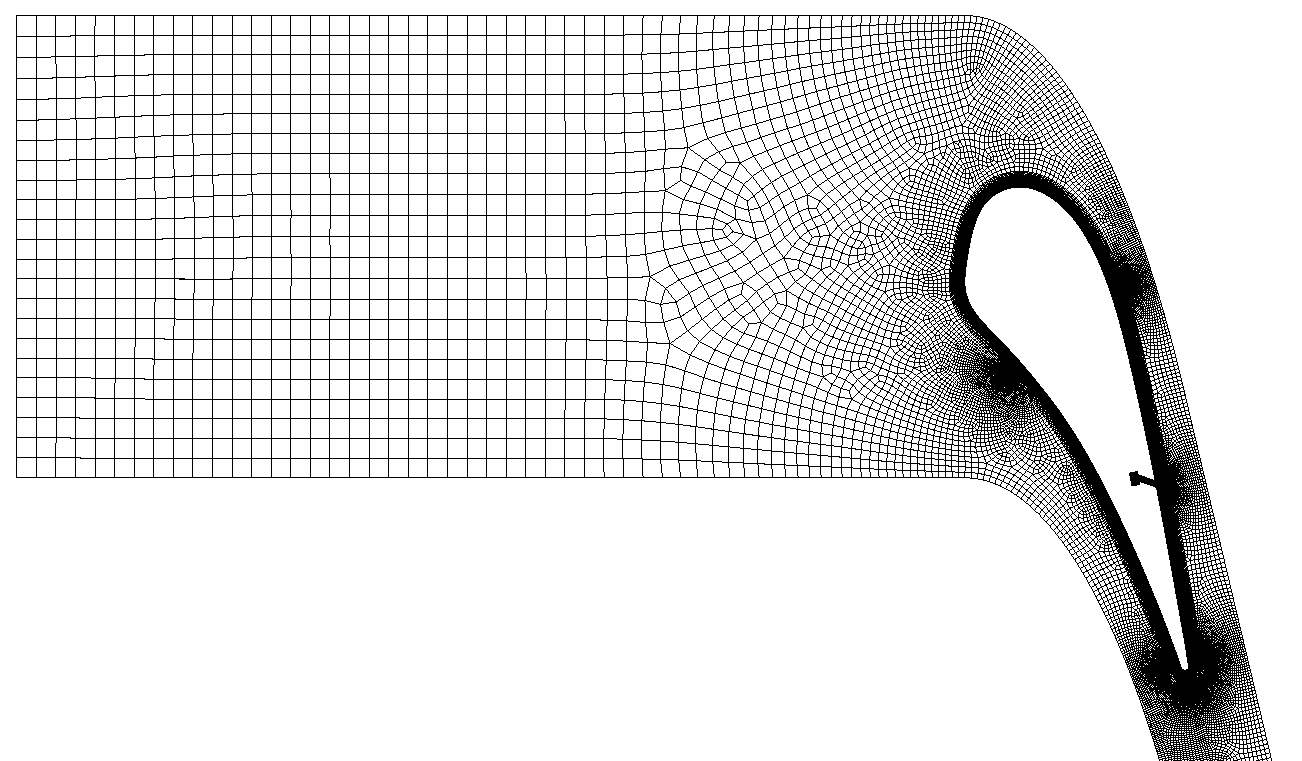
\includegraphics[width=\linewidth]{figs/SCH_mesh_domain_placeholder.png}
    \caption{XWB mesh for NGV and upstream domain}
    \label{fig:SCH_mesh_1}
  \end{subfigure}
  \vspace{0.05\textwidth}
  \begin{subfigure}{.45\textwidth}
    \centering
    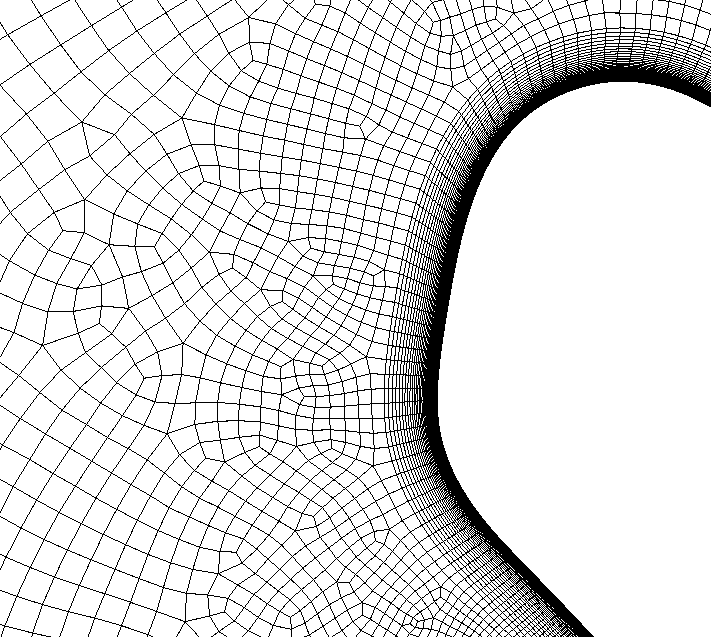
\includegraphics[width=\linewidth]{figs/SCH_mesh_leading_edge_placeholder.png}
    \caption{XWB mesh for leading edge}
    \label{fig:SCH_mesh_2}
  \end{subfigure}
  \hspace{0.05\textwidth}
  \begin{subfigure}{.45\textwidth}
    \centering
    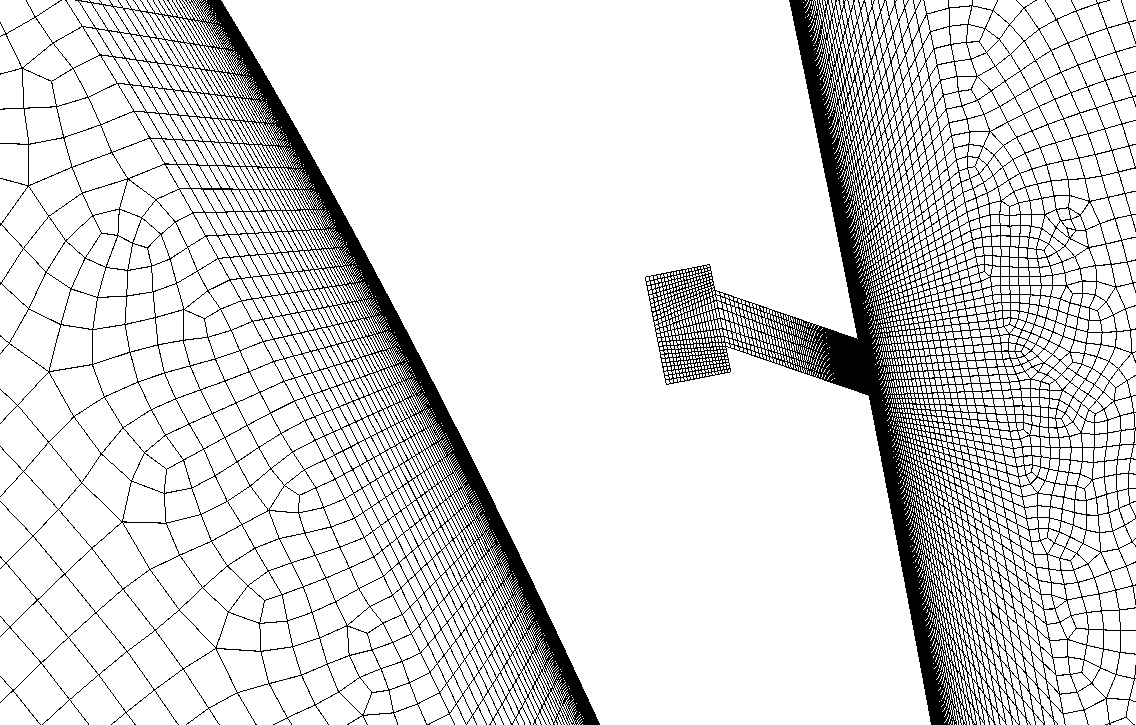
\includegraphics[width=\linewidth]{figs/SCH_mesh_hole_placeholder.png}
    \caption{XWB mesh for cooling hole and plenum}
    \label{fig:SCH_mesh_3}
  \end{subfigure}
  \caption{Details of mesh for XWB single cooling hole study}
\end{figure}

\textcolor{red}{Review the literature for why correctly modelling turbulence is important for capturing the mainstream/coolant mixing, and thus why two turbulence models are compared.}

\textcolor{red}{Plot capacity changes versus hole position and discuss its causes, mentioning the literature reviewed in the chapter intro (plus the two definitions of capacity where coolant is concerned - which one is used in earlier chapters??) A maximum ~0.5 percent change in capacity resulted from an unrealistically drastic shifting of a 2D cooling slot along the vane's suction side.}
\begin{figure}[H]
      \centering
      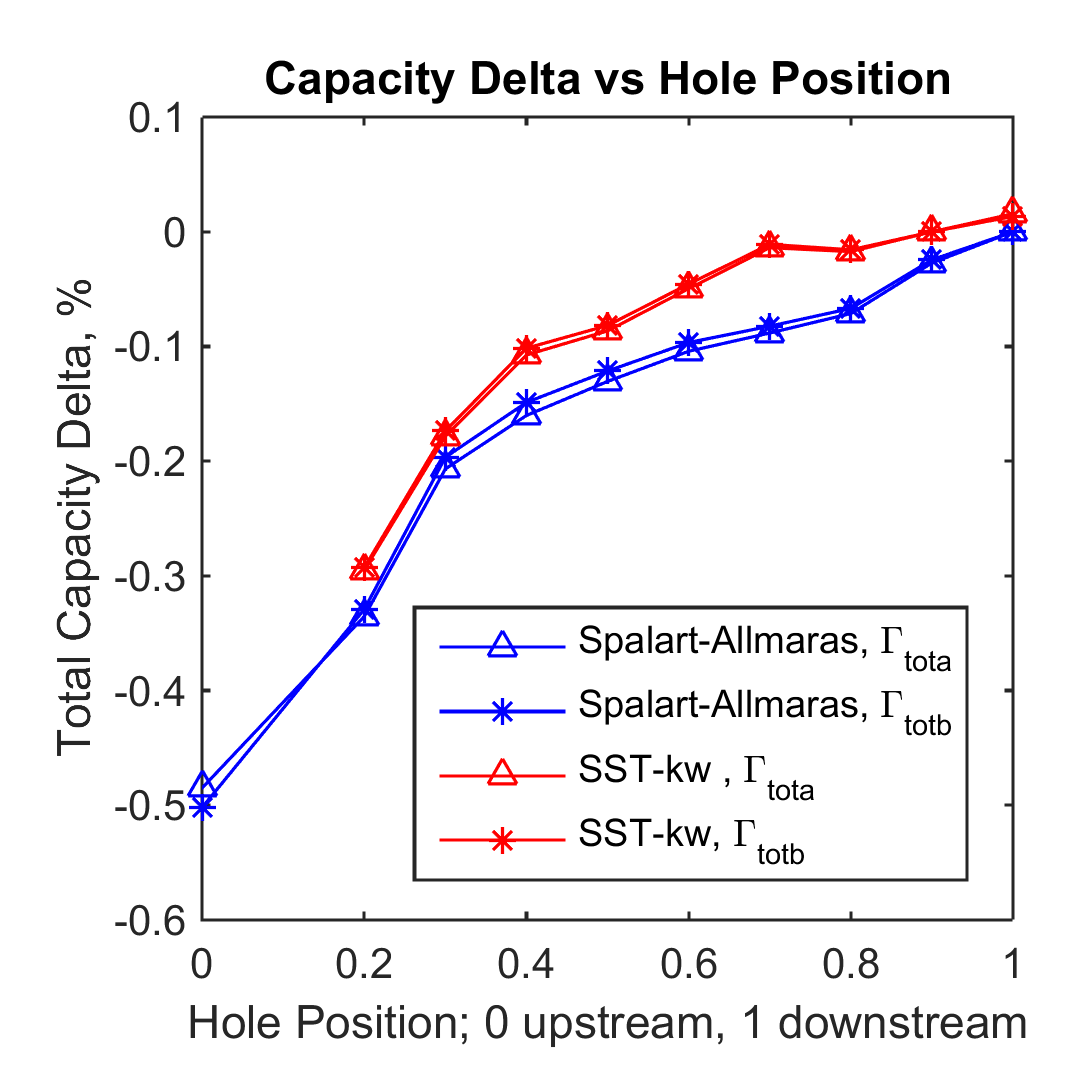
\includegraphics[width=.45\textwidth]{figs/SCH_capacity_vs_hole_position.png}
      \caption{Total capacity percentage delta as a function of single cooling hole position}
      \label{fig:SCH_capacity_vs_hole_position}
\end{figure}

\textcolor{red}{Things that might be driving the change in capacity, and that can be examined from the existing data:}
	\textcolor{red}{Changing boundary layer thickness causing a change in effective throat area}

    
\section{Consideration of corrections necessary to interpret 2D result}

\textcolor{red}{Different:}

\textcolor{red}{Mass flow rate between a 2D slot and a 3D row of holes}

\textcolor{red}{Mixing between coolant and mainstream}

\textcolor{red}{Angle of ejection}

\textcolor{red}{Papers about matching the conditions when simulating a cooling row:}

\textcolor{red}{S. Ravelli - NUMERICAL ASSESSMENT OF DENSITY RATIO AND MAINSTREAM TURBULENCE EFFECTS ON LEADING EDGE FILM COOLING: HEAT AND MASS TRANSFER METHODS~\cite{ravelli_engine_conditions}}
		\textcolor{red}{Arguing: In a CFD simulation of four film cooling hole rows, the usual parameters (DR, BR, MFR, TuI) aren't enough to ensure you have matched the engine conditions}
		\textcolor{red}{Raw data: A previous experimental study (PSP) to validate their CFD, and their CFD}
		\textcolor{red}{I discuss: Criticise my own signle cooling slot work - is it really representative enough for its capacity effects to be predictable}
		\textcolor{red}{I also cite: Other CFD on film cooling}
		\textcolor{red}{My raw data: My single cooling row data, emphasis on the CFD parameters and setup}
		
\textcolor{red}{Giovanna Barigozzi - Experimental investigation of the interaction between showerhead coolant jets and main flow~\cite{barigozzi_film_cooling}}
		\textcolor{red}{Arguing: When film coolant is ejected upstream , observed high turbulence and velocity fluctuations suggest the mixing is a random process without coherent structures, and unsteady, and 3D}
		\textcolor{red}{Raw data: Their experimental study, including pressure-sensitive paint and particle-image velocimetry}
		\textcolor{red}{I discuss: Do we know less than we thought about how much film coolant is actually getting to the LE SS? Reason why you might want an extra row there? Also, clear support for my arguing that proper CFD investigations of SS LE film cooling should not be a 2D slot and should not be steady}
		
\textcolor{red}{Wei He - Film cooling and aerodynamic performances of a turbine nozzle guide vane with trenched cooling holes~\cite{he_film_cooling}}
		\textcolor{red}{Arguing: A novel design for film cooling holes, using a zigzag-shaped trench, has some advantages but is only really suitable for the middle PS}
		\textcolor{red}{Raw data: Their 3D CFD on a single-vane linear cascade, where the trench moves around various positions}
		\textcolor{red}{I discuss: They mention BR etc, relevant to me. Their movable trench is a bit like my movable 2D slot, except it is mainly confined to the PS, whereas mine is on the SS. But my quasi-3D study could be easily adapted to repeat their study of the novel trench shape}
		\textcolor{red}{My raw data: My Q3D study}



\addcontentsline{toc}{chapter}{Bibliography}
\bibliographystyle{ieeetr}
\bibliography{tmfg_bibliography_ver01}



\end{document}
